% BEGIN PREAMBEL
\documentclass[9pt, xcolor=dvipsnames]{beamer}
\usepackage[british]{babel}
\usepackage{multimedia}
\usepackage{amsmath,amsfonts,amssymb}
\usepackage{upgreek}
\usepackage{pgfpages}
\usepackage[version=3]{mhchem}
\usepackage{lmodern}
\usepackage{graphicx}
\usepackage{multicol}
\usepackage{color}
\usepackage{xcolor,fontawesome}
\usepackage{wrapfig}
\usepackage{siunitx}
\usepackage{fontspec}
\usepackage{tikz}
\usepackage{textpos}
\usepackage{booktabs}
\usepackage{caption}
\usepackage{subcaption}
\usepackage{wasysym}
\usepackage{animate}
\usepackage{tabularx}
\usepackage{ETHlogo}
\newfontfamily\ubuntu{Ubuntu}
\newcommand{\as}{\\[14pt]}
\newcommand{\s}{\\[7pt]}
\newcommand{\is}{\\[2pt]}
\newcommand{\no}{\noindent}
\newcommand{\ka}{\hspace*{0.5cm}}
\newcommand{\ma}{\hspace*{1cm}}
\newcommand{\ga}{\hspace*{1.5cm}}
\newcommand{\li}{\left|}
\newcommand{\re}{\right|}
\newcommand{\const}{\text{const.}}
\newcommand{\z}{\text}
\newcommand{\terminal}[1]{\colorbox{black}{\textcolor{white}{{\fontfamily{phv}\selectfont \scriptsize{#1}}}}}
\newcommand{\plugin}[1]{\textit{\flq#1\frq}}
\newcommand{\ra}{$\rightarrow$ }
\definecolor{cadmiumgreen}{rgb}{0.0, 0.42, 0.24}
\newcommand{\itemfill}{\setlength{\itemsep}{\fill}}
\newcommand{\orderof}[1]{$\mathcal{O}\left(#1\right)$}
\usetheme{Boadilla}
\graphicspath{ {Pics/} }
\makeatletter
\def\input@path{ {sections/} }
\makeatother
\usecolortheme[named=ForestGreen]{structure}
\useoutertheme{miniframes}
\beamertemplatenavigationsymbolsempty
\makeindex
\author[M. Reichmann]{Michael Reichmann}
\institute[\textbf{\textit{ETH}}\scalebox{.6}{\textit{Z\"{u}rich}}]{Swiss Federal Institute of Technology Zurich}
\AtBeginSection{\frame[noframenumbering]{\sectionpage}}

\setbeamercolor{frametitle}{bg=date in head/foot.bg!20!white}

%% TITLE PAGE
\defbeamertemplate*{title page}{customized}[1][] {
	\ETHlogo[3cm]
	\vspace*{-33pt}
	\begin{figure}[t]
		\flushright
		
\includegraphics[height=.9cm]{IPP}
	\end{figure}
	\vspace*{-10pt}
	\begin{figure}
		\centering
		\includegraphics[height=.4\textheight]{\inserttitlegraphic}
	\end{figure}
	\begin{block}{}
		\centering
		\vspace*{1pt}
		\usebeamerfont{title}\usebeamercolor[fg]{title}\textbf{\inserttitle}\\\vspace*{5pt}
		\usebeamerfont{subtitle}\insertsubtitle\\\vspace*{1pt}
	\end{block}
	\vspace*{10pt}
	\centering
	\color{black}
	\usebeamerfont{author}\textbf{\insertauthor}\par\vspace*{5pt}
	\usebeamerfont{date}\insertdate\par
}

%% FOOTLINE
\setbeamertemplate{footline}
{
  \leavevmode%
  \hbox{%
  \begin{beamercolorbox}[wd=.3\paperwidth,ht=2.25ex,dp=1ex,center]{author in head/foot}%
    \usebeamerfont{author in head/foot}\insertshortauthor\hspace*{2pt}
    (
\includegraphics[height=3.5pt]{ETHLogoWhite})
  \end{beamercolorbox}%
  \begin{beamercolorbox}[wd=.4\paperwidth,ht=2.25ex,dp=1ex,center]{title in head/foot}%
    \usebeamerfont{title in head/foot}\insertshorttitle
  \end{beamercolorbox}%
  \begin{beamercolorbox}[wd=.3\paperwidth,ht=2.25ex,dp=1ex,right]{date in head/foot}%
    \usebeamerfont{date in head/foot}\insertdate\hspace*{3em}
    \insertframenumber{} / \inserttotalframenumber\hspace*{1ex}
  \end{beamercolorbox}}%
  \vskip0pt%
}
 
%% SECTION PAGE
\setbeamertemplate{section page}
{
    \begin{centering}
		\usebeamerfont{title}Section \insertsectionnumber\\\vspace*{.7cm}
		\begin{beamerboxesrounded}[shadow=true, lower=frametitle]{}
			\centering
			\vspace*{3pt}
			\usebeamerfont{frametitle}\textbf{\insertsection}\par
			\vspace*{3pt}
		\end{beamerboxesrounded}
    \end{centering}
}

\title[short]{Overview of the PhD Project}
\subtitle{ETH Group Meeting}
\titlegraphic{PixTel}
% END PREAMBEL

\begin{document}

% ============= TITLE PAGE =============
\usebackgroundtemplate{\tikz\node[opacity=0.2] {\hspace*{-5pt}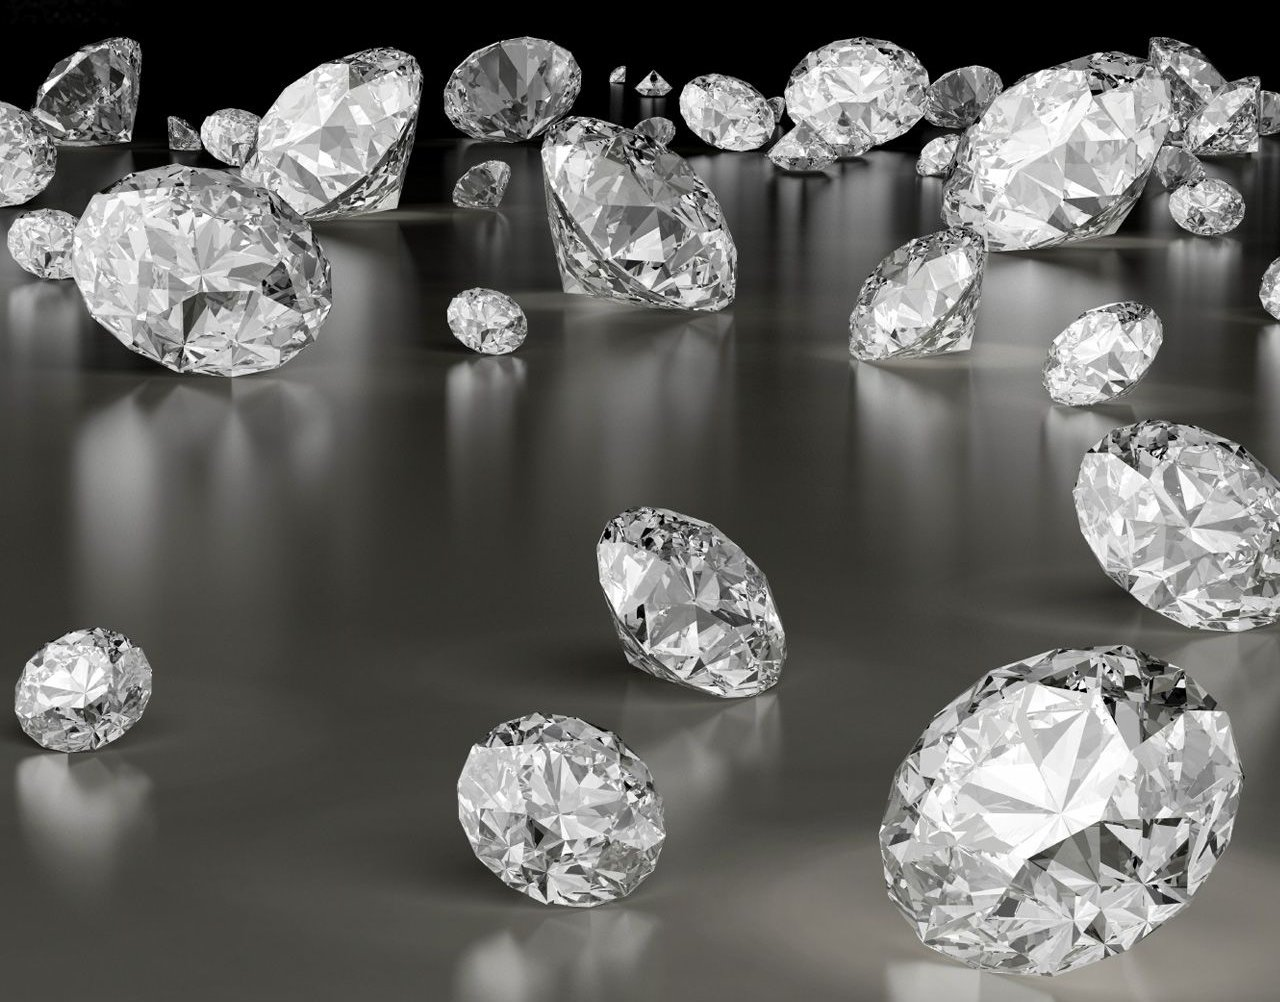
\includegraphics[height=\paperheight,width=1.05\paperwidth]{bkg.jpg}};}
\maketitle
\usebackgroundtemplate{}

% ============= TABLE OF CONTENTS ======
\begin{frame}%[allowframebreaks]
	\frametitle{Table of contents}
	\tableofcontents[hideallsubsections]   % [pausesections]
\end{frame}

% ============= 1 =============
\section{Introduction}
\begin{frame}{Introduction}

	\textbf{\underline{Time Line:}}\vspace*{5pt}
	\begin{itemize}
		\itemfill
		\item $2015/02 - 2015/08$: Master Thesis at IPP 
		\item $2015/08 - 2016/01$: Scientific assistant
		\item $2016/02 - \z{today}$: \hspace*{7.5pt} PhD Student
	\end{itemize}\vspace*{10pt}
	
	\uncover<2->{
		\textbf{\underline{Projects:}}\vspace*{5pt}
		\begin{itemize}
			\itemfill
			\item \usebeamercolor[fg]{title}\textbf{Rate dependence of diamond as detector material}
			\begin{itemize}
				\itemfill\usebeamercolor[fg]{normal text}
				\item commissioning, supervision and further development of the ETH beam telescope
				\item pad detectors
				\item pixel detectors
				\item 3D detectors (pad \& pixel)
				\item supervision and organisation of beam tests
			\end{itemize}\vspace*{5pt}

			\item \usebeamercolor[fg]{title}\textbf{CMS Pixel Layer 1 \ra pROC}
			\begin{itemize}
				\itemfill\usebeamercolor[fg]{normal text}
				\item Layer 1 software
				\item high rate beam tests
				\item L1 readout errors
			\end{itemize}
		\end{itemize}}

\end{frame}


% ============= 2 =============
\section{Motivation}
\begin{frame}{Motivation}

	\begin{itemize}
		\item innermost layers \ra highest radiation damage
		\item current detector is designed to survive \SI{\sim12}{month} in High-Luminosity LHC
		\item \usebeamercolor[fg]{title} \textbf{\ra R/D for more radiation hard detector designs and/or materials}
	\end{itemize}\vspace*{10pt}
	
	\uncover<2->{
		\textbf{\underline{Diamond as Detector Material:}}\vspace*{5pt}
		\begin{itemize}
			\itemfill
			\item advantageous properties 
			\begin{itemize}
				\itemfill
				\item radiation hardness
				\item isolating material
				\item high charge carrier mobility
			\end{itemize}
		\end{itemize}}

	\uncover<3->{
		\begin{itemize}
			\item diamond pixel detectors in Pixel Luminosity Telescope (PLT) (installed 2010/2011)
			\item \textcolor{RedOrange}{\textbf{signal dependence on incident particle rate observed!}}
		\end{itemize}}
	
	\uncover<4->{
		\begin{itemize}
			\item investigation of the rate effect in various detector designs:
			\begin{itemize}
				\itemfill
				\item pad \ra full diamond as single cell readout of the whole signal
				\item pixel \ra diamond sensor on CMS-Pixel Chips
				\item 3D \ra pixel detector with clever design to reduce drift distance
			\end{itemize}

		\end{itemize}}
		
\end{frame}

% ============= 3 =============
\section{Diamond Types}
\begin{frame}{Artificial Diamond Types}

	\begin{itemize}
		\item diamonds artificially grown with chemical vapour deposition (CVD)
		\item investigation of two different diamond types:
	\end{itemize}
	
	\begin{figure}[h] 
		\centering
		\begin{subfigure}{0.45\textwidth}  
			\centering
			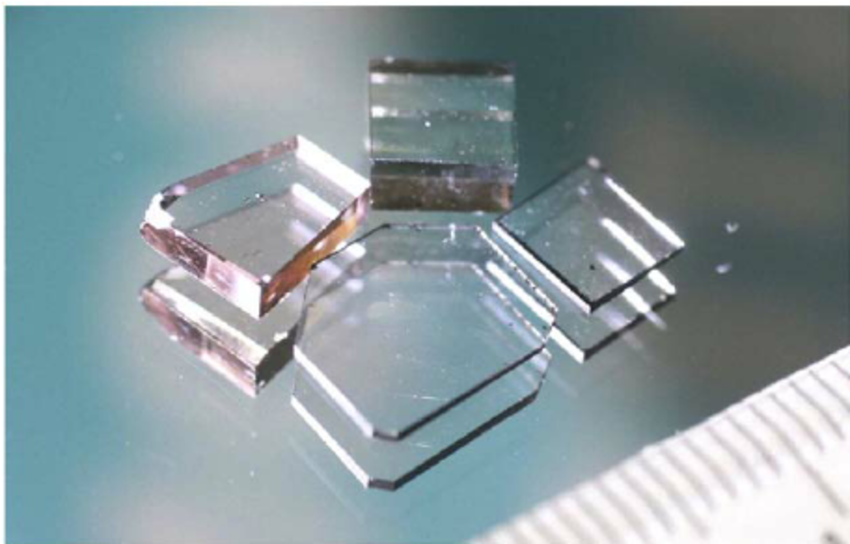
\includegraphics[height=0.4\textheight]{SCVD}
			\caption{single-crystalline CVD}
		\end{subfigure}
		\begin{subfigure}{0.45\textwidth} 
			\centering
			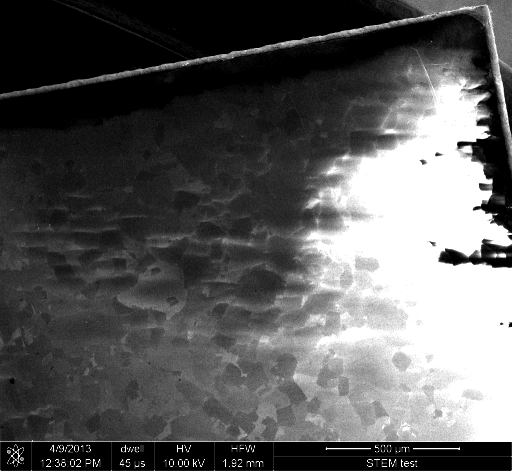
\includegraphics[height=0.4\textheight]{pCVD4}
			\caption{poly-crystalline CVD} 	
		\end{subfigure} 
	\end{figure}
	
	\begin{minipage}{5.5cm}
		\begin{itemize}
			\item grown on existing diamond crystal
			\item only small sizes (\SI{\sim.25}{cm^2})
			\item larger signals than pCVD ($5:3$)
		\end{itemize}
	\end{minipage}
	\hspace*{.5cm}
	\begin{minipage}{5cm}
		\begin{itemize}
			\item grown on Si substrate with diamond powder
			\item large wafers (\SIrange{5}{6}{''} \diameter)
			\item non-uniformities and grains
		\end{itemize}
	\end{minipage}
	
\end{frame}


% ============= 4 =============
\section{Test Site \& Setup}
\begin{frame}{Test Site}

	\begin{itemize}
		\itemfill
		\item High Intensity Proton Accelerator (HIPA) at PSI (Cyclotron)
		\item using beam line $\uppi$M1 at Paul Scherrer Institute (PSI)
		\item positive pions ($\uppi^+$) with momentum of \SI{260}{\mega\electronvolt\per c} 
		\item tunable particle fluxes from \orderof{\SI{1}{\kilo\hertz\per cm^2}} to \orderof{\SI{10}{\mega\hertz\per cm^2}}
	\end{itemize}
	
	\begin{figure}
		\centering
		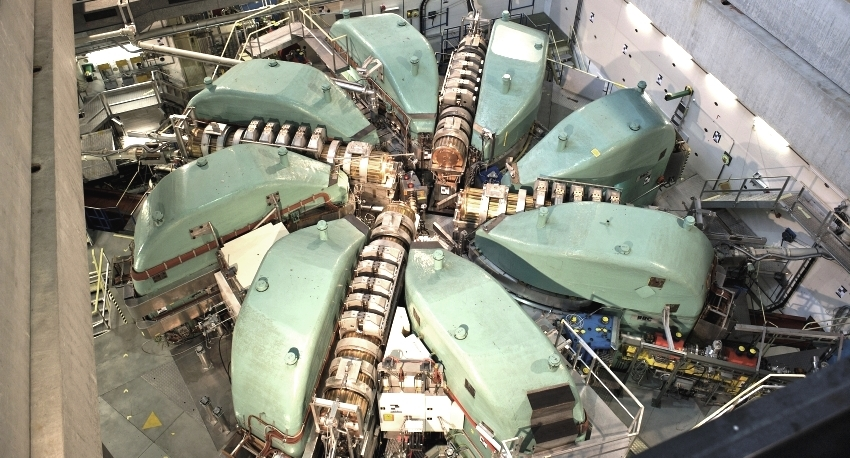
\includegraphics[width=6.5cm]{cyclotron}
	\end{figure}
		
\end{frame}
% ================================ 2 ========================================
\begin{frame}{Setup}
 
	\begin{figure}
		\centering
		\only<1>{
			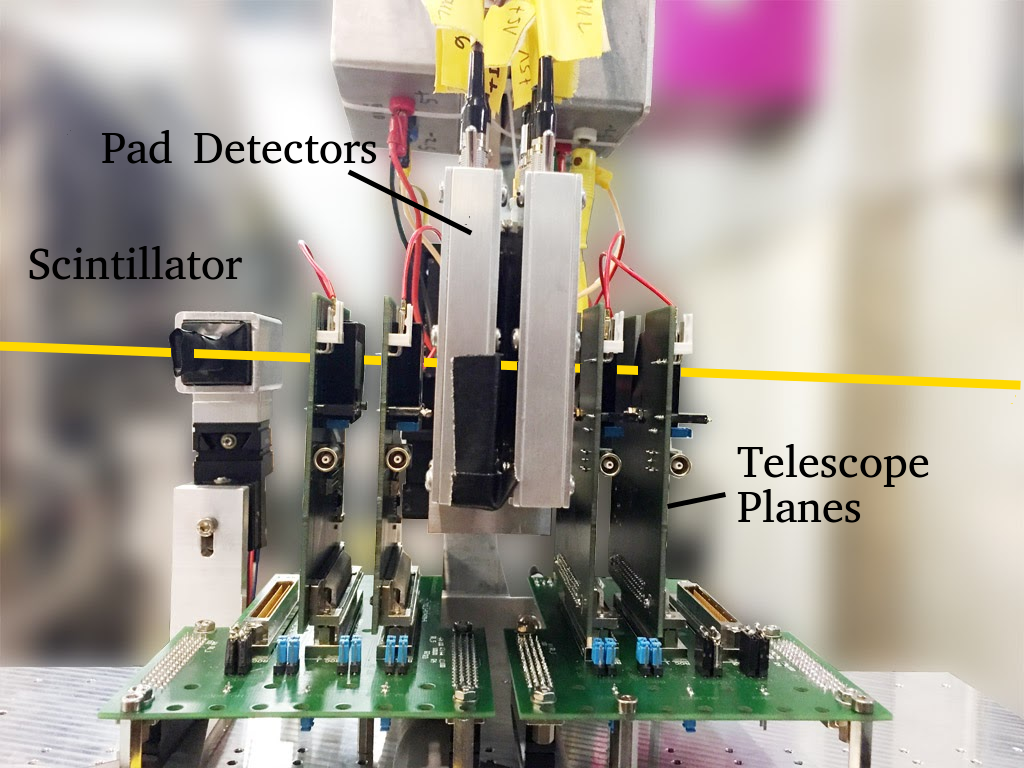
\includegraphics[height=.4\textheight]{Setup}
			\caption{pad telescope}}
		\only<2>{
			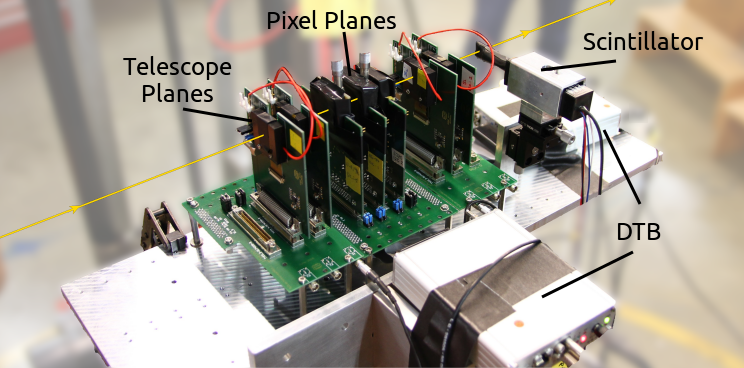
\includegraphics[height=.4\textheight]{PixTel1}
			\caption{pixel telescope}}
	\end{figure}\vspace*{-5pt}
 
	\begin{itemize}
		\itemfill
		\item modular ETH beam telescope \ra test apparatus for all detectors
		\item 4 tracking planes \ra trigger (fast-OR) with scalable area
		\item fast-OR clocked with \SI{40}{\mega\hertz} \ra \SI{25}{\nano\second} time precision
		\item diamond detectors (DUTs) in between tracking planes
		\item scintillator for precise trigger timing \ra \orderof{\SI{1}{\nano\second}}
	\end{itemize}

\end{frame}

% ================================ 3 ========================================
\begin{frame}{Setup}
 
	\begin{figure}
		\centering
		\only<1>{
			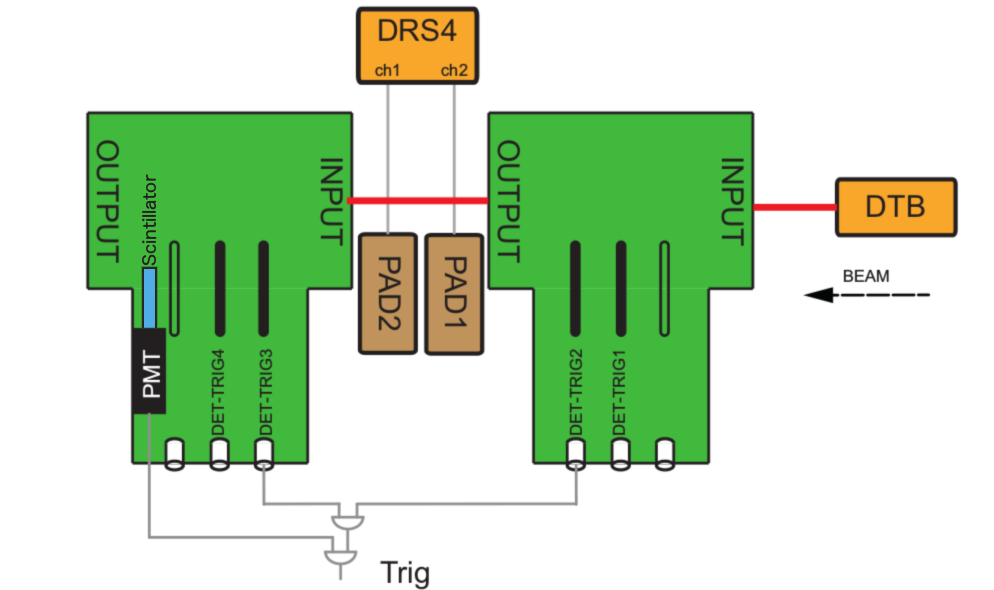
\includegraphics[height=.4\textheight]{SchematicsV2}
			\caption{pad telescope}}
		\only<2>{
			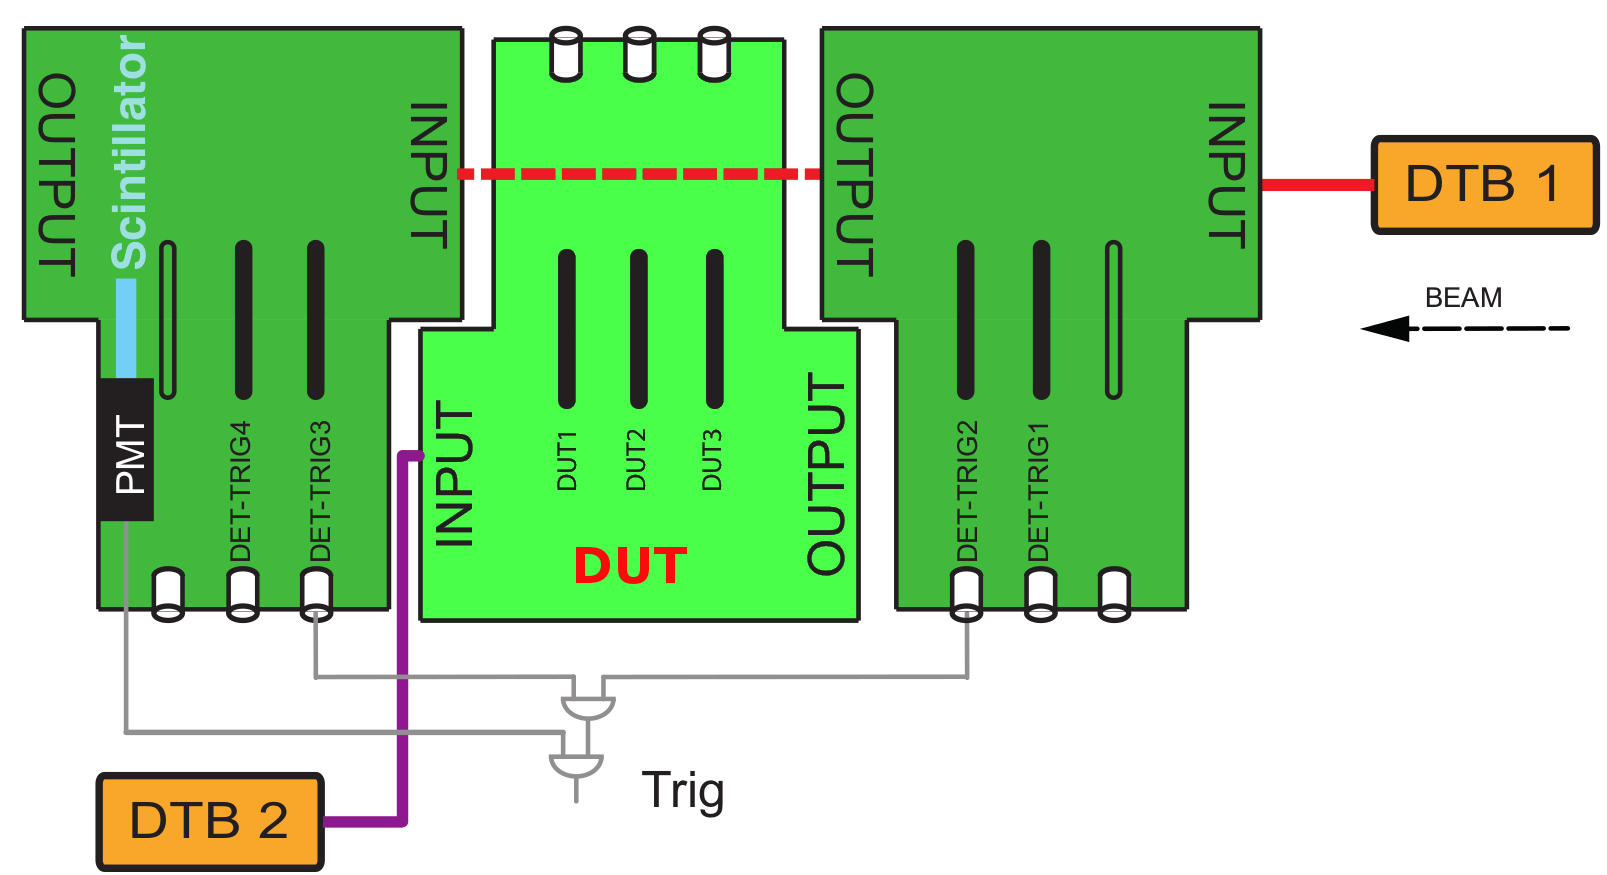
\includegraphics[height=.4\textheight]{TelSchemePix}
			\caption{pixel telescope}}
	\end{figure}\vspace*{-5pt}
 
	\begin{itemize}
		\itemfill
		\only<1>{\item PSI DRS4 Evaluation Board as digitizer for the pad waveforms}
		\only<2>{\item independent telescope module as DUT (light green)}
		\item Digital Test Board (DTB) and pXar software for the telescope readout
		\item global trigger as coincidence of fast-OR self trigger and scintillator signal
		\item EUDAQ as DAQ framework
	\end{itemize}

\end{frame}





% ============= 5 =============
\section{Pad Detectors}
\begin{frame}{Pad Detectors}

	\begin{figure}[h] 
		\centering
		\begin{subfigure}{0.45\textwidth}  
			\centering
			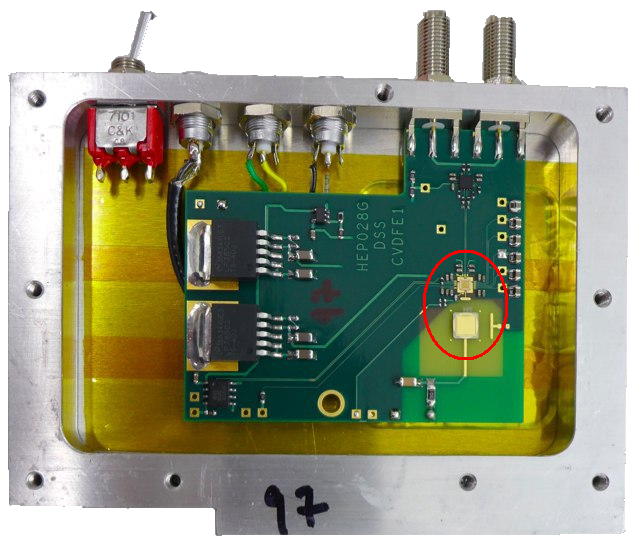
\includegraphics[height=0.45\textheight]{PadBox}
			\caption{fast amplifier box}
		\end{subfigure}
		\begin{subfigure}{0.45\textwidth} 
			\centering
			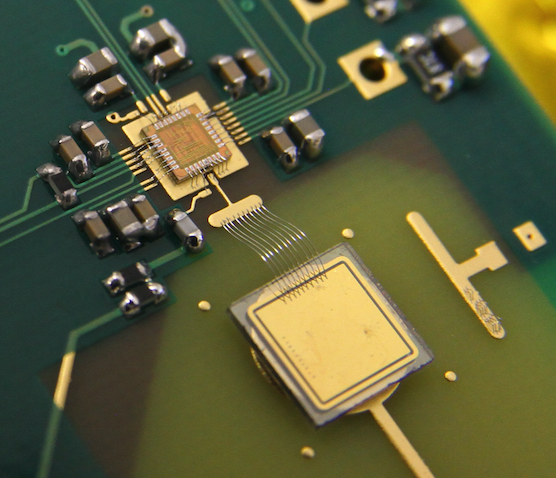
\includegraphics[height=0.45\textheight]{PadFull}
			\caption{diamond and fast amp} 	
		\end{subfigure} 
	\end{figure}
	
	\begin{itemize}
		\itemfill
		\item diamonds in custom built amplifier boxes from Ohio State University (OSU)
		\item cleaning, photo-lithography and Cr-Au metallisation at OSU
		\item low gain, fast amplifier with \orderof{\z{ns}} rise time
	\end{itemize}
	
\end{frame}
% ============================ FRAME 2 ==========================================>
\begin{frame}
	\frametitle{Waveforms}
	\vspace*{-20pt}
	\begin{center}
		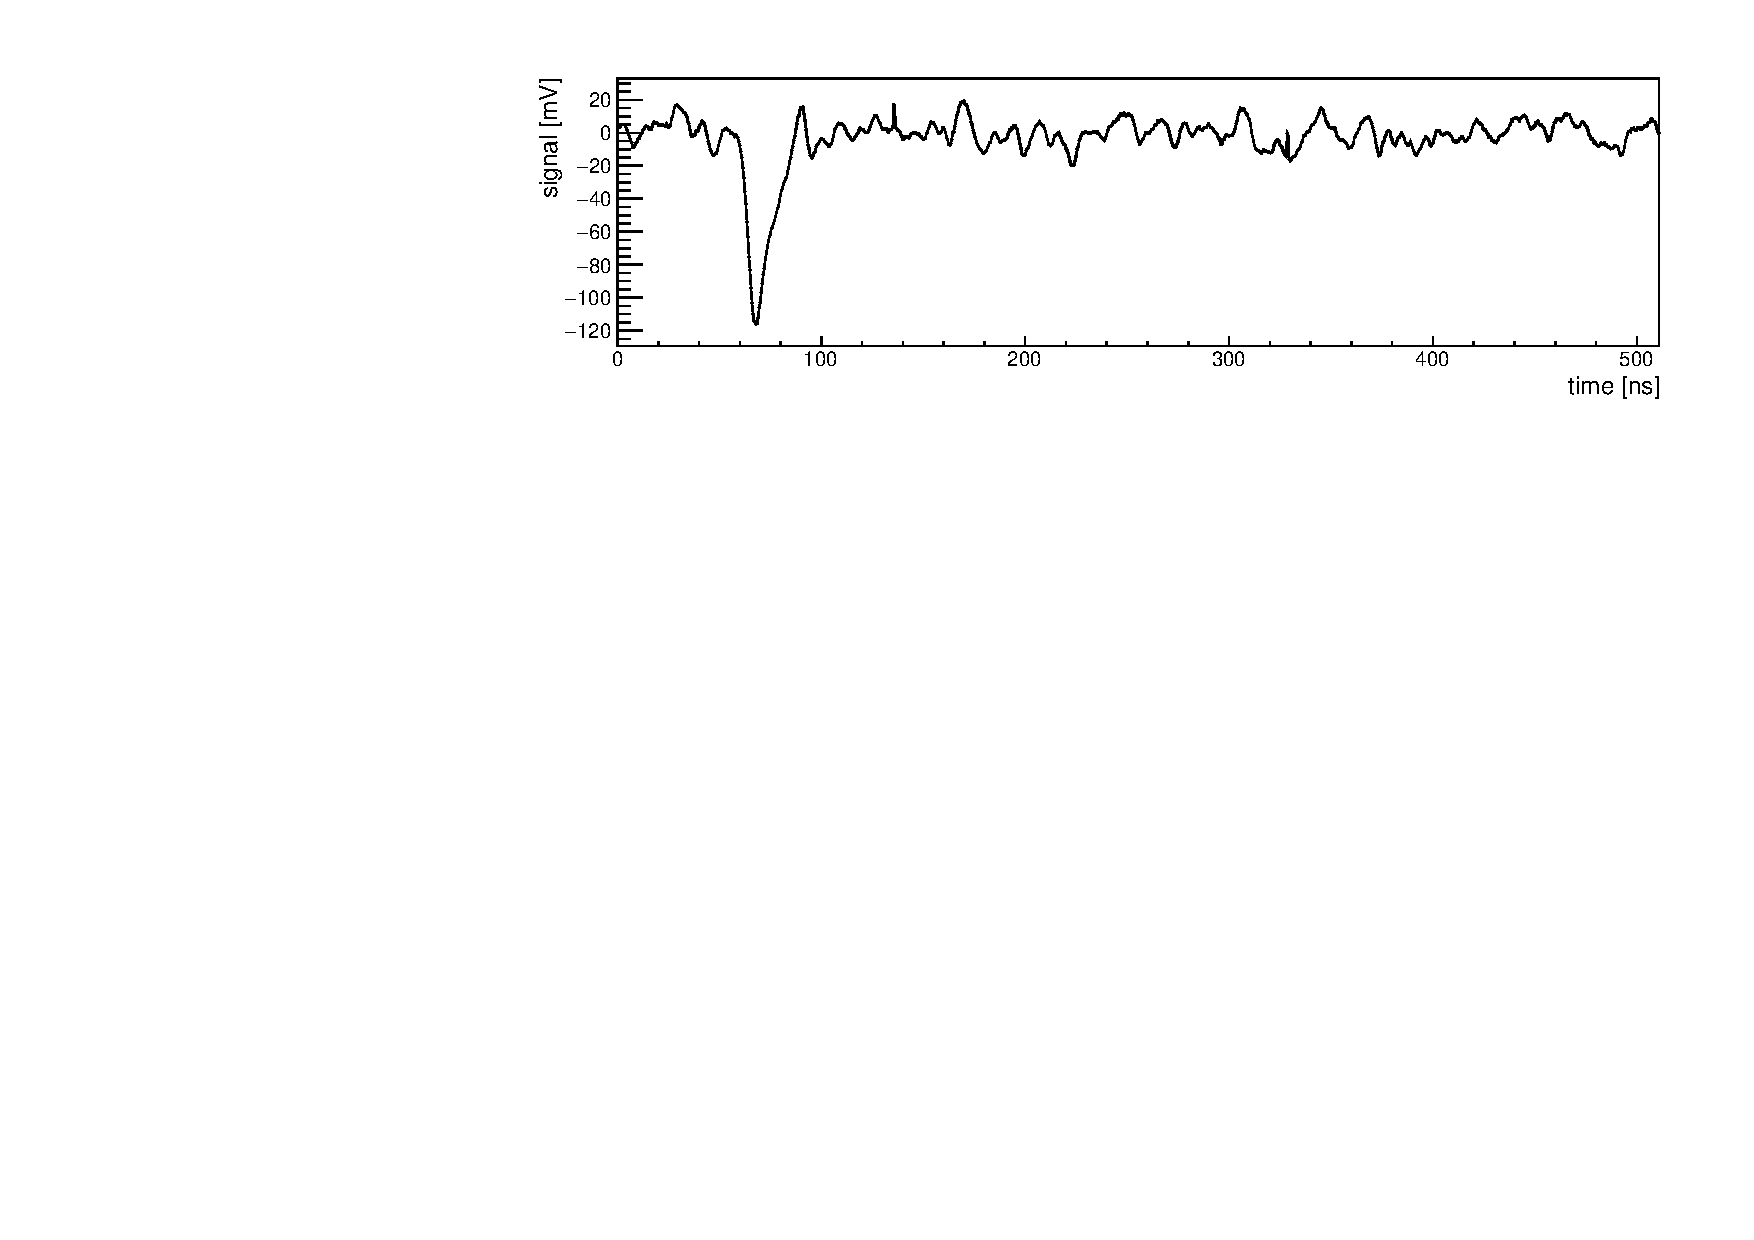
\includegraphics[angle=270, width=.7\textwidth]{SignalWaveform}\\
		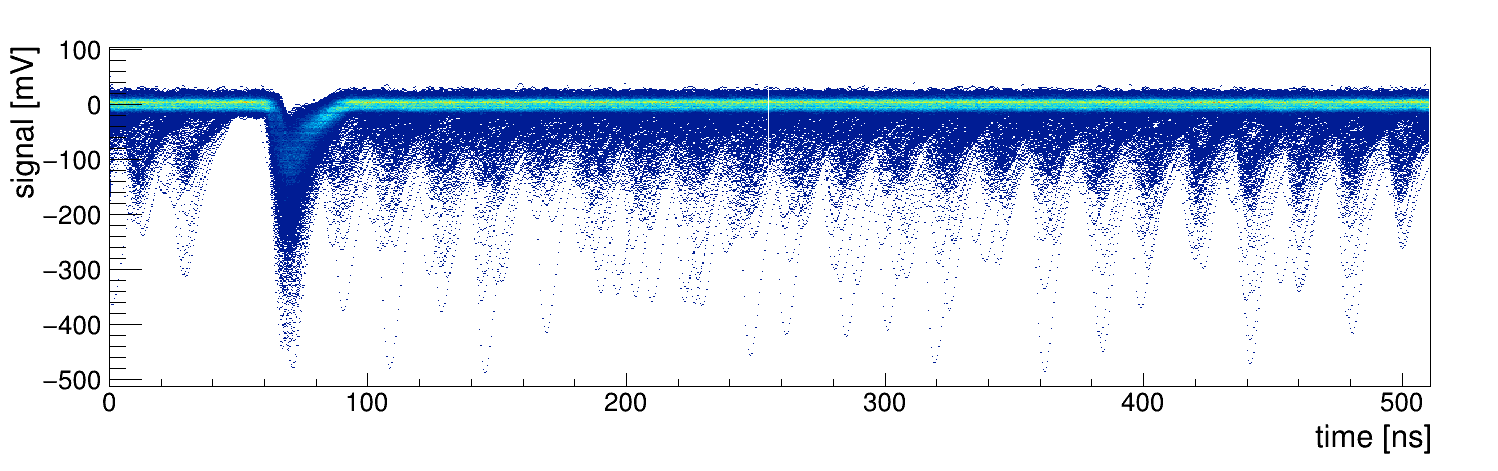
\includegraphics[width=.7\textwidth]{SignalWaveforms5000}
	\end{center}
	\begin{itemize}
		\item most frequented peak (\SI{\sim70}{ns}): triggered signal
		\item other peaks originate from other buckets ($\rightarrow$ resolve beam structure of \SI{\approx19.7}{ns})
		\item system does not allow signals in pre-signal bucket due to fastOR trigger deadtime
	\end{itemize}
\end{frame}
% ============================ FRAME 3 ==========================================>
\begin{frame}
	\frametitle{Pulse Height Calculation}
	\vspace*{-5pt}
	\begin{center}
		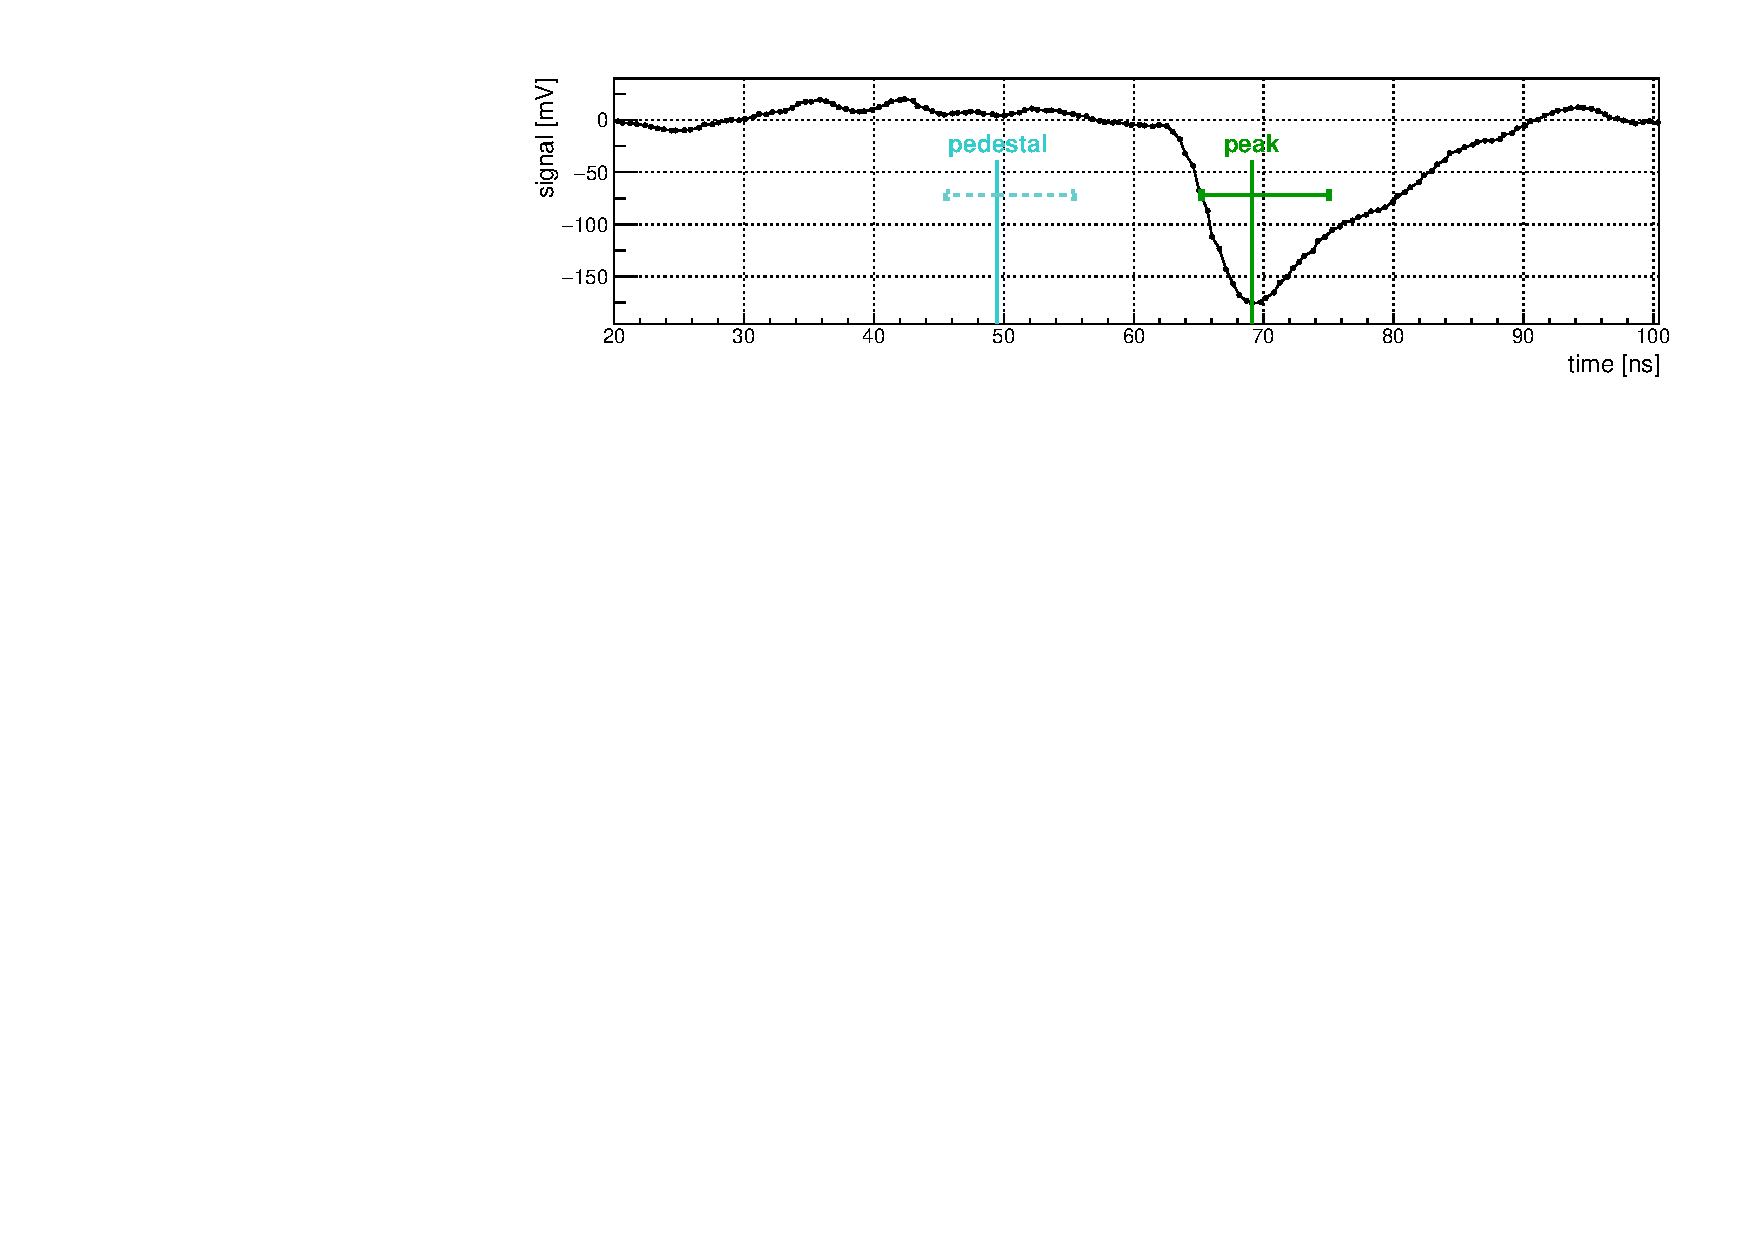
\includegraphics[angle=270, width=\textwidth]{intpeaks}\\
	\end{center}
	\vspace*{-5pt}
	\begin{itemize}
		\setlength{\itemsep}{\fill}
		\item finding the peak in the signal region
		\item integrating the signal in time fixed asymmetric integral around peak
		\item optimising the integral width by highest SNR (Integral / Pedestal Sigma)
	\end{itemize}
\end{frame}
% ============================ FRAME 4 ==========================================>
\begin{frame}
	\frametitle{Non-Irradiated Single Crystal Diamond}
	\def \sp {3.7cm}
	\begin{minipage}{\sp}
		\centering
		October 2015 
		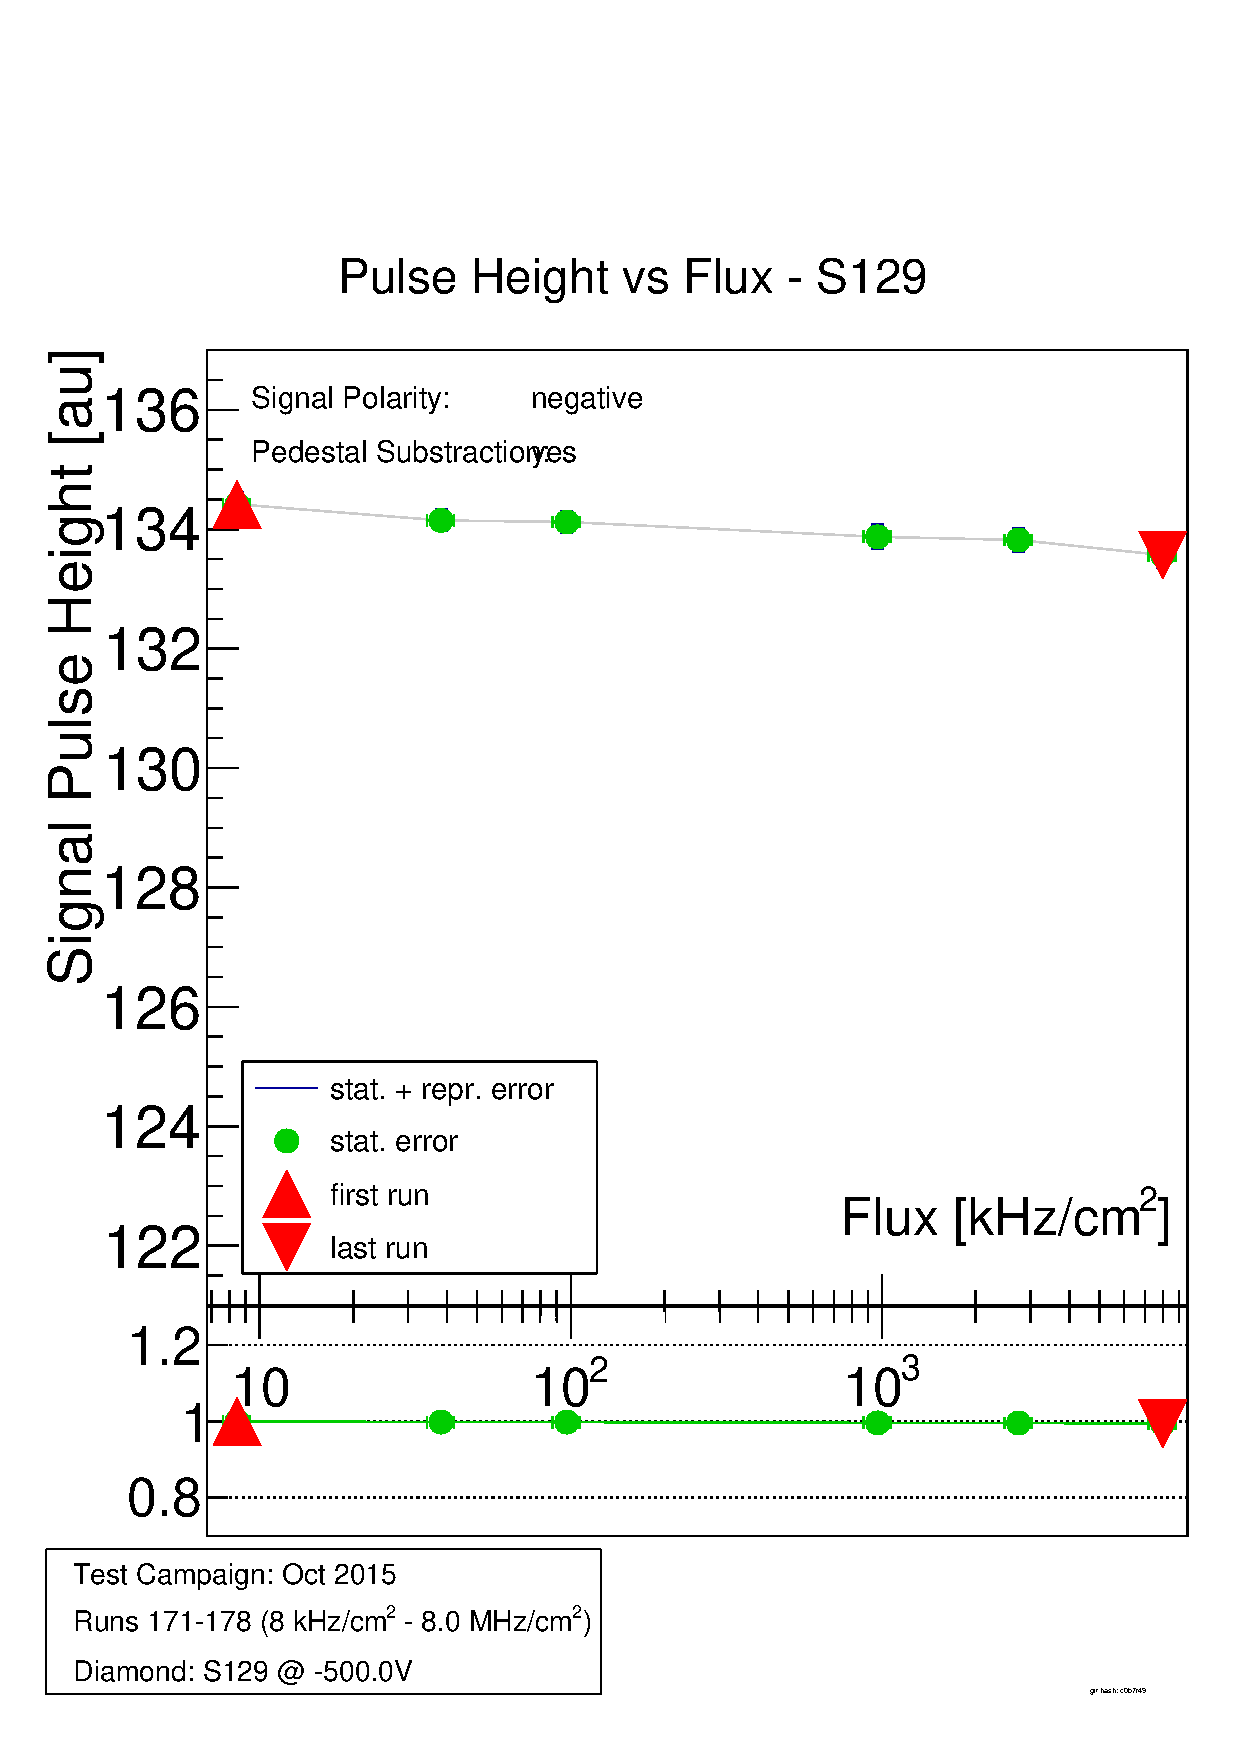
\includegraphics[width=\sp]{S129Oct15}\\
		noise $\upsigma\approx$ \SI{2.6}{au}
	\end{minipage}
	\hspace*{2pt}
	\begin{minipage}{\sp}
		\centering
		August 2016
		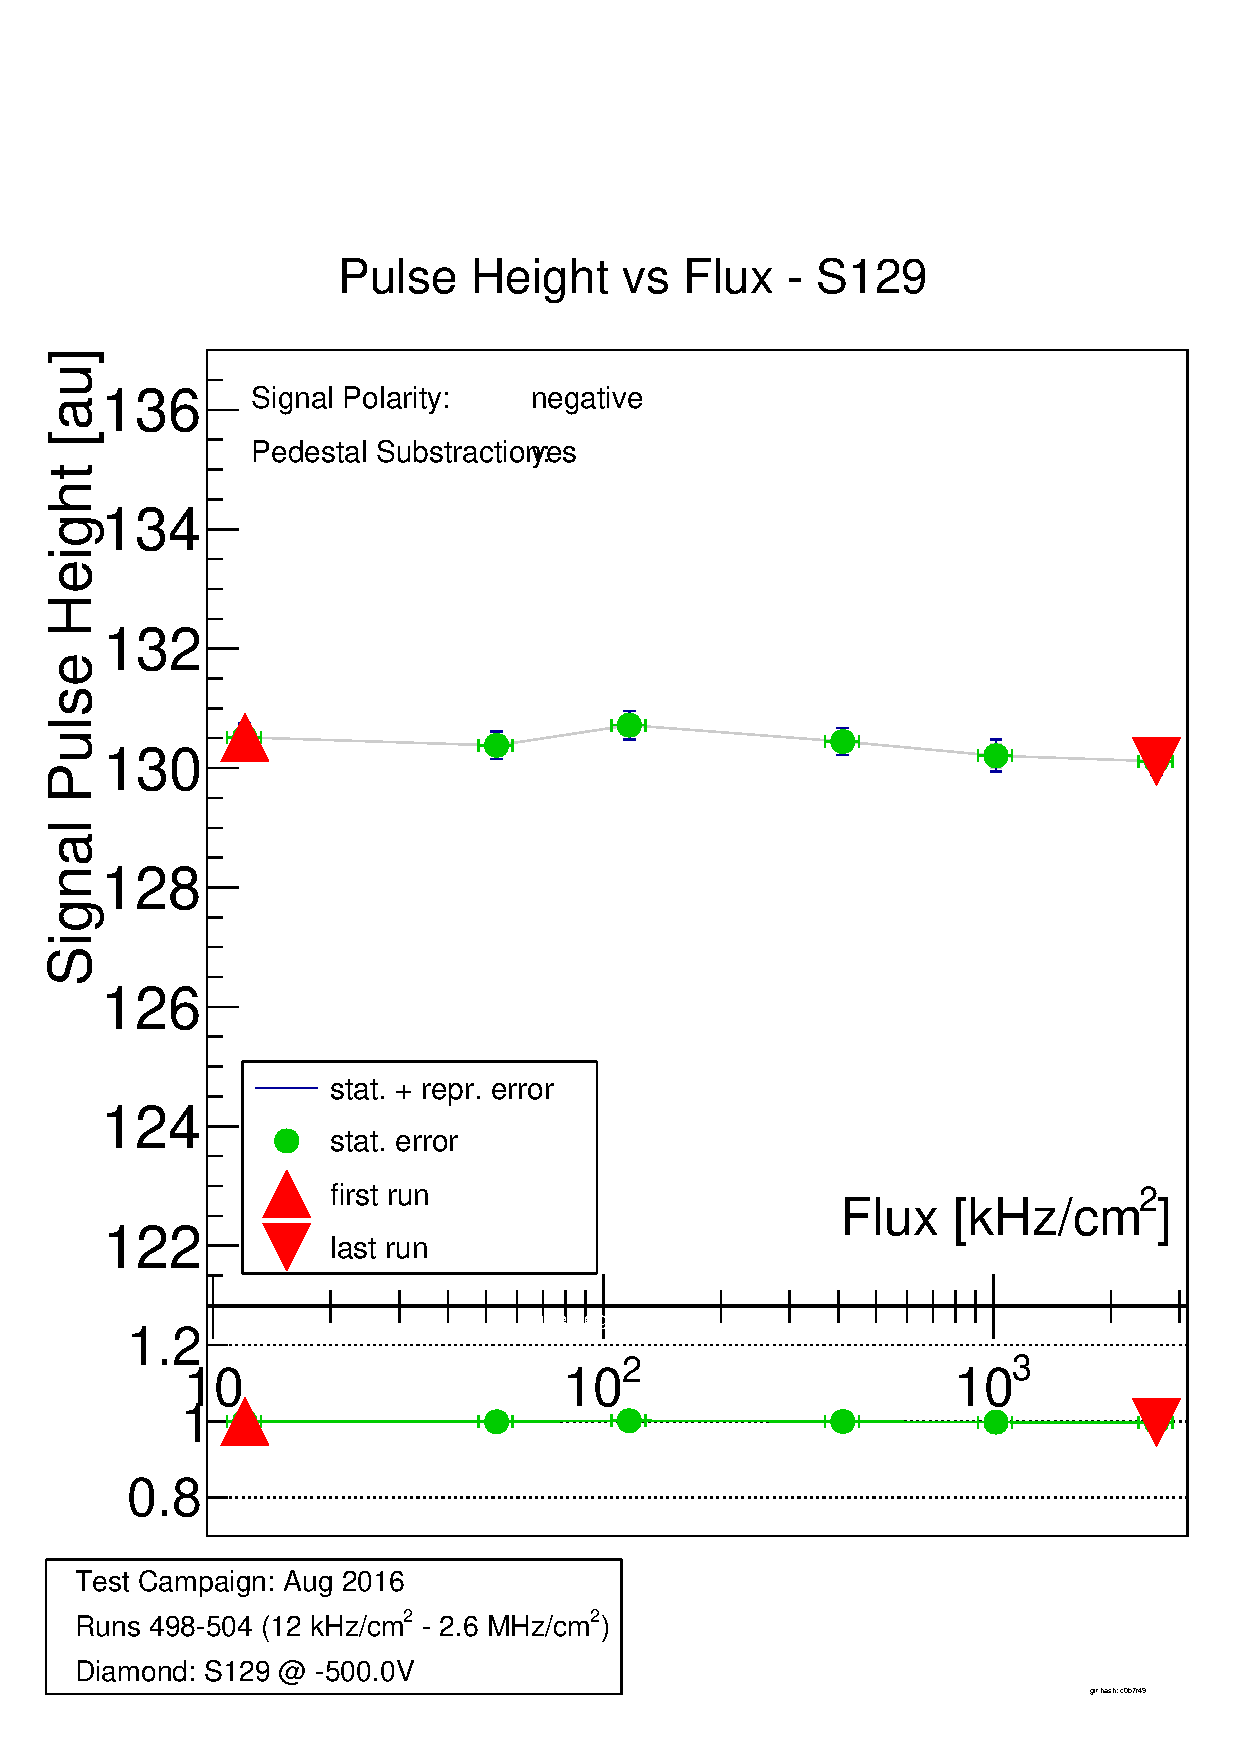
\includegraphics[width=\sp]{S129Aug16}\\
		noise $\upsigma\approx$ \SI{2.6}{au}
	\end{minipage}
	\hspace*{2pt}
	\begin{minipage}{\sp}
		\centering
		October 2016
		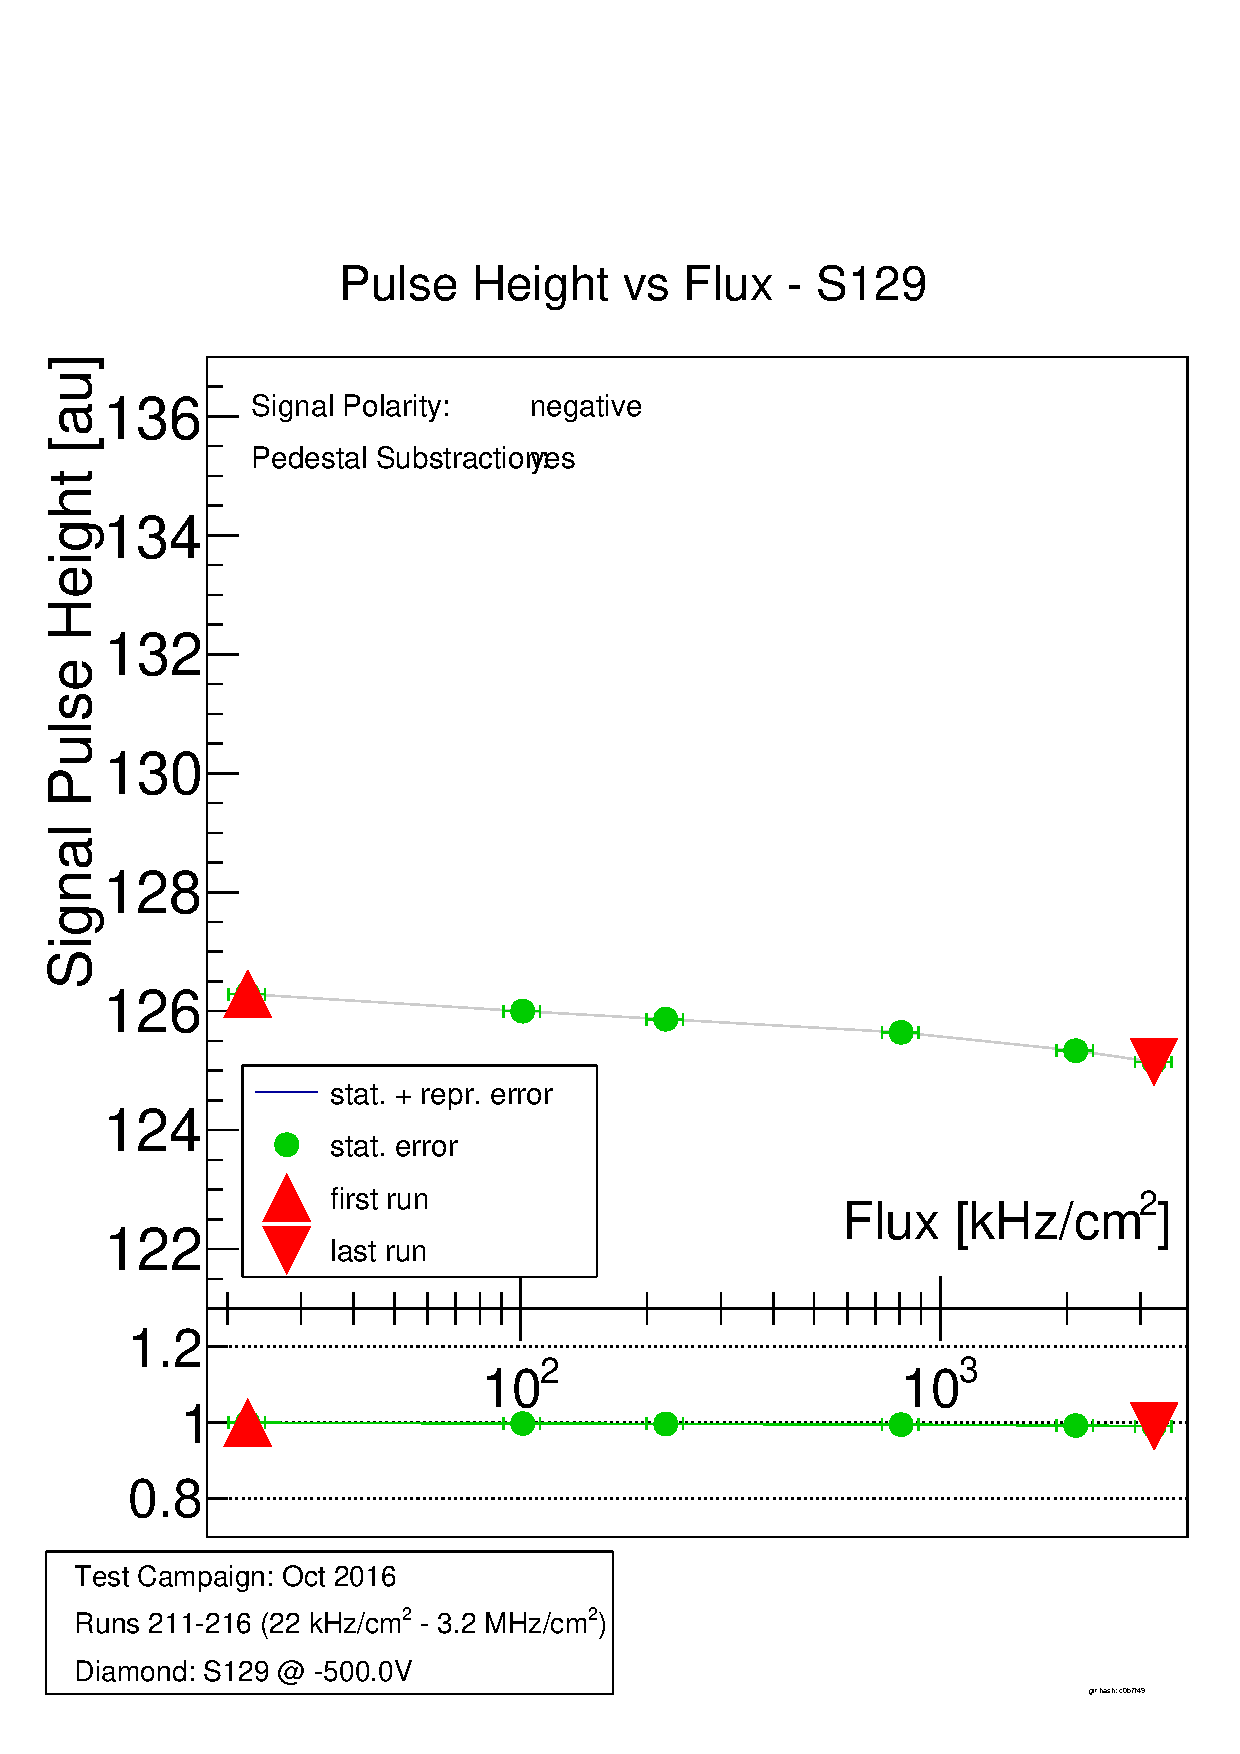
\includegraphics[width=\sp]{S129Oct16}\\
		noise $\upsigma \approx$ \SI{2.6}{au}
	\end{minipage}\s
	\begin{itemize}
		\item measurements taken under the same conditions
		\item noise stays the same
		\item pulse height very stable
	\end{itemize}
\end{frame}
% ============================ FRAME 5 ==========================================>
\begin{frame}
	\frametitle{Poly Crystal Diamond}
	\begin{minipage}{2.8cm}
		\centering
		August 2016 - \\unirradiated
		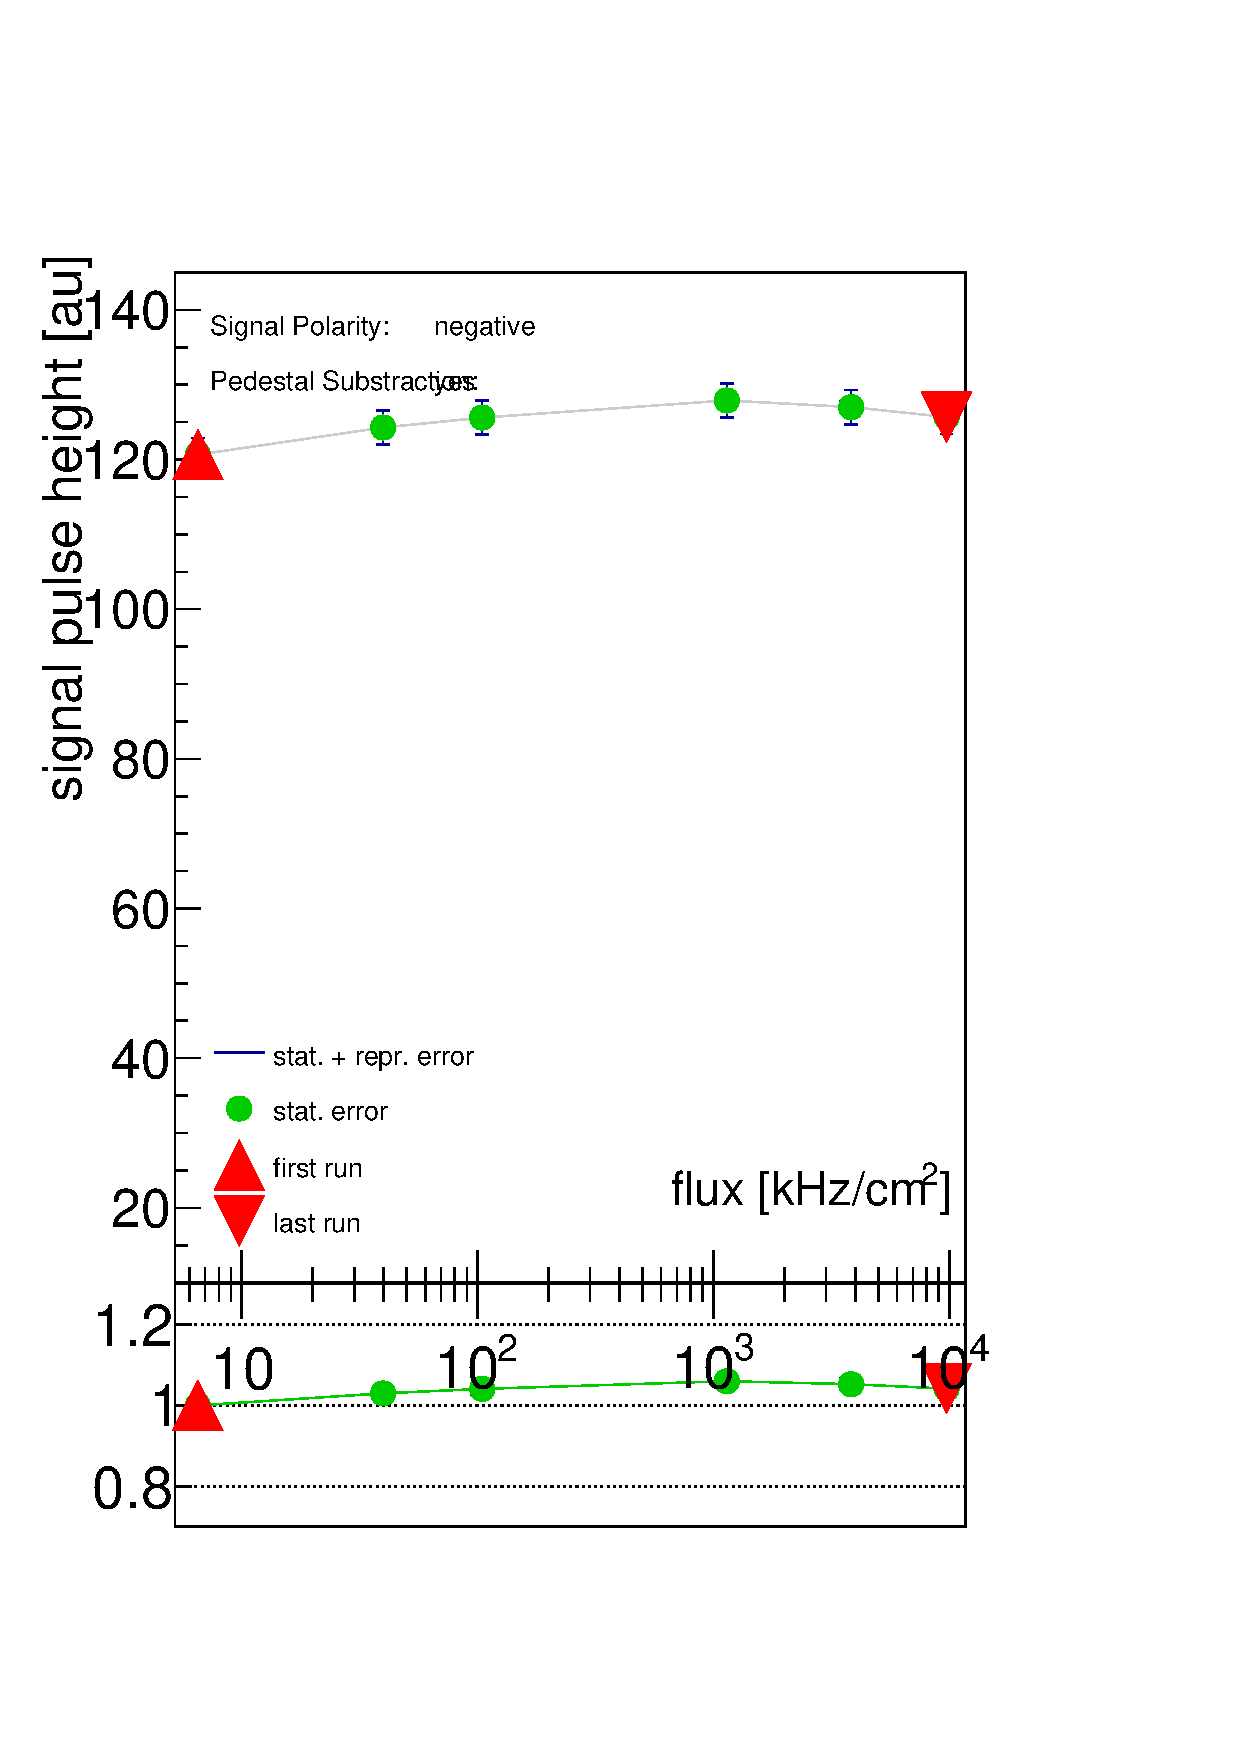
\includegraphics[width=3cm]{CPH1508_13_2.pdf}\\
		noise $\upsigma\approx$ \SI{4.9}{au}
	\end{minipage}
	\hspace*{2pt}
	\begin{minipage}{2.8cm}
		\centering
		October 2015 - \SI[exponent-product = \cdot]{5e14}{n/cm^{2}}
		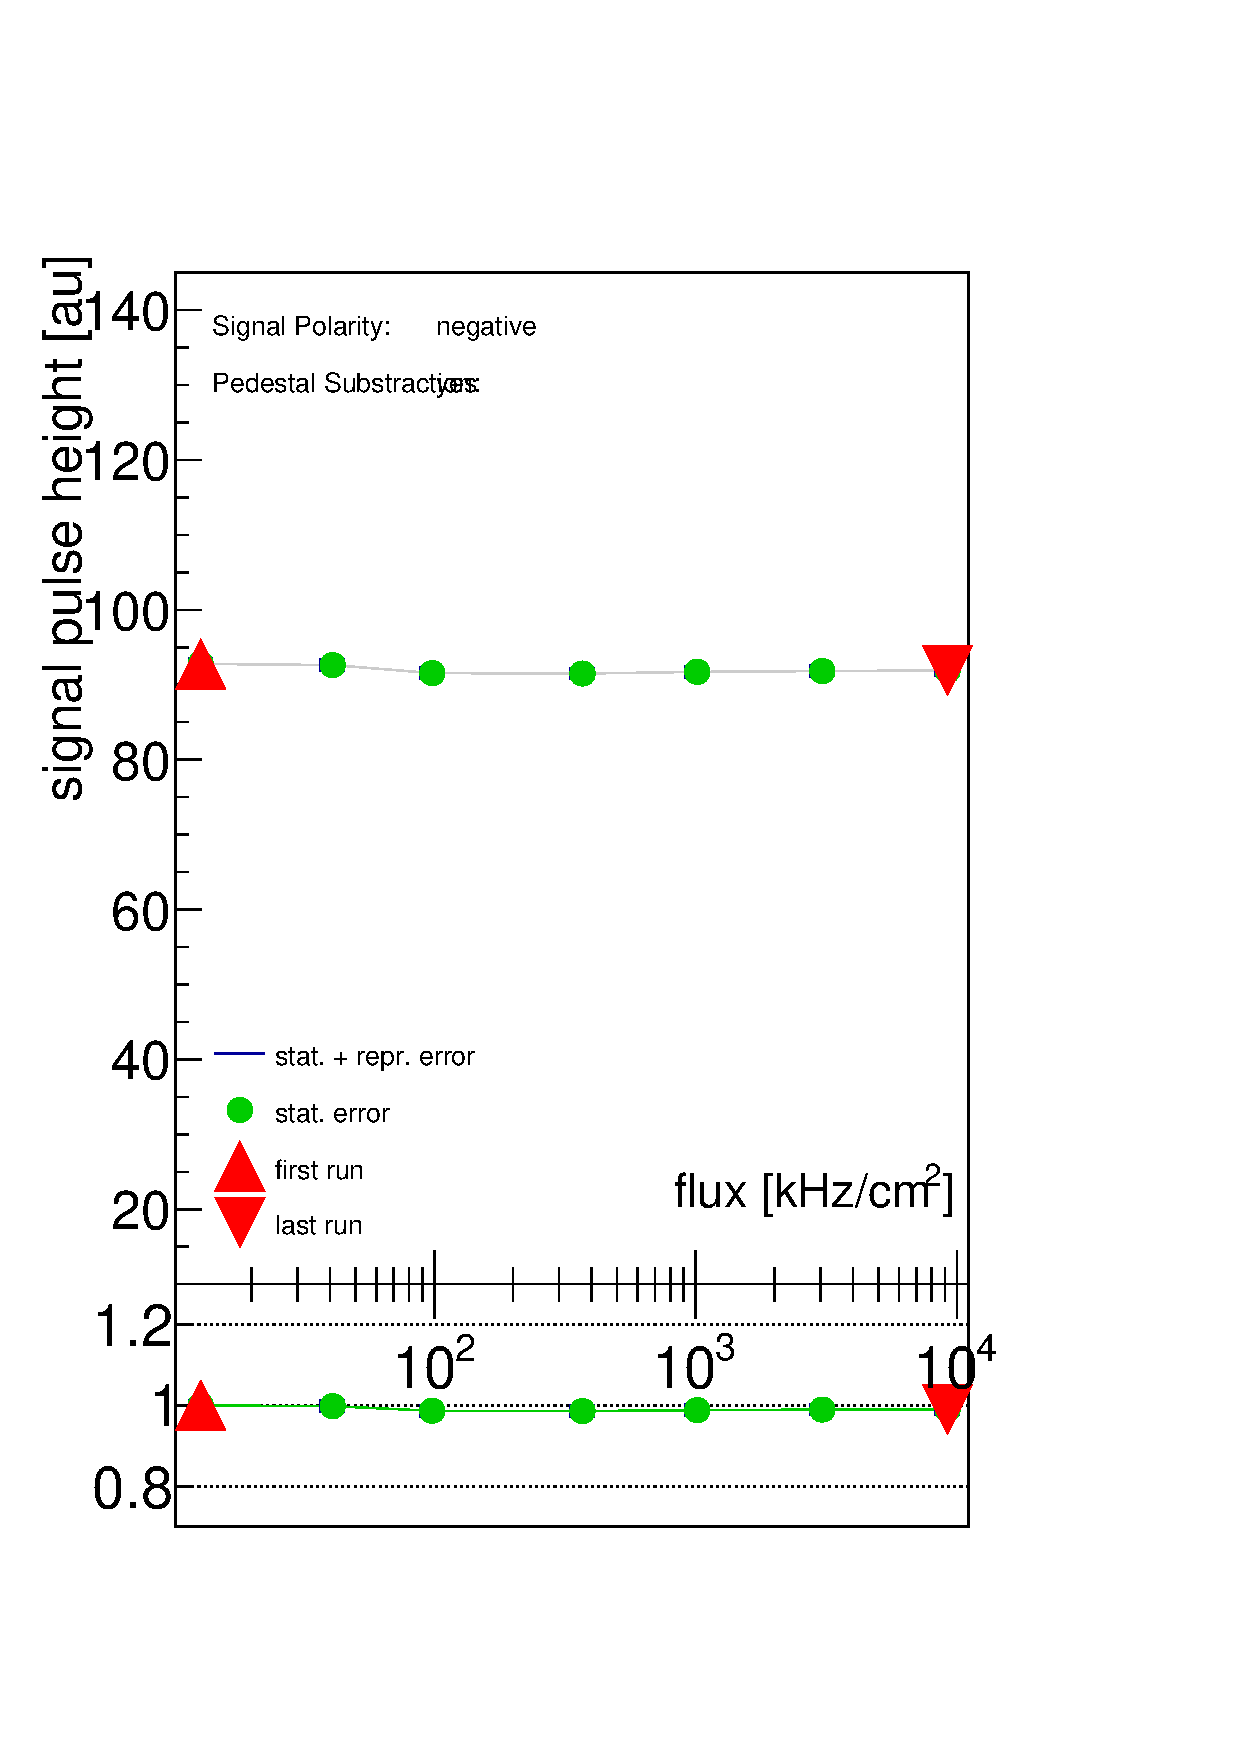
\includegraphics[width=3cm]{CPH1510_08_2.pdf}\\
		noise $\upsigma\approx$ \SI{4.9}{au}
	\end{minipage}
	\hspace*{2pt}
	\begin{minipage}{2.8cm}
		\centering
		August 2016 - \SI[exponent-product = \cdot]{1e15}{n/cm^{2}}
		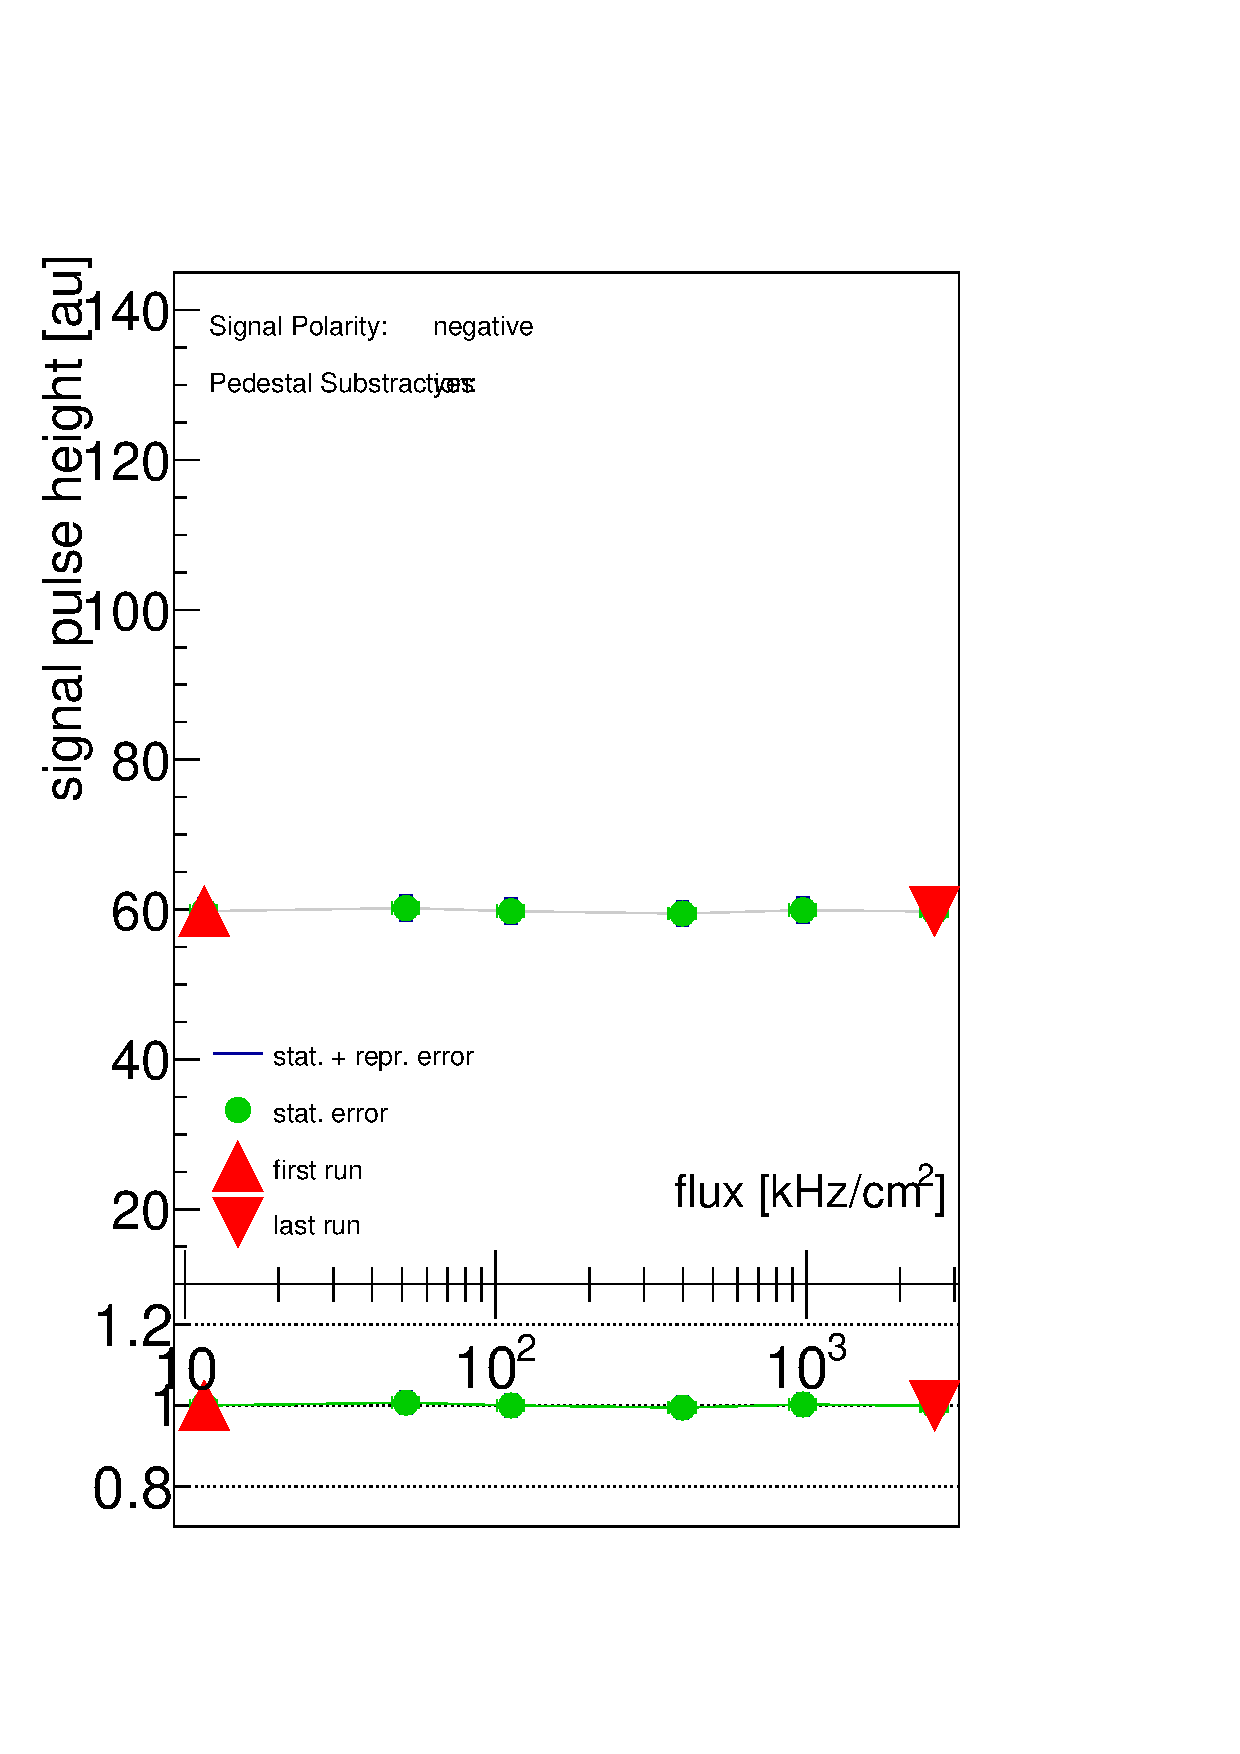
\includegraphics[width=3cm]{CPH1608_09_1.pdf}\\
		noise $\upsigma \approx$ \SI{4.9}{au}
	\end{minipage}
	\hspace*{2pt}
	\begin{minipage}{2.8cm}
		\centering
		October 2016 - \SI[exponent-product = \cdot]{2e15}{n/cm^{2}}
		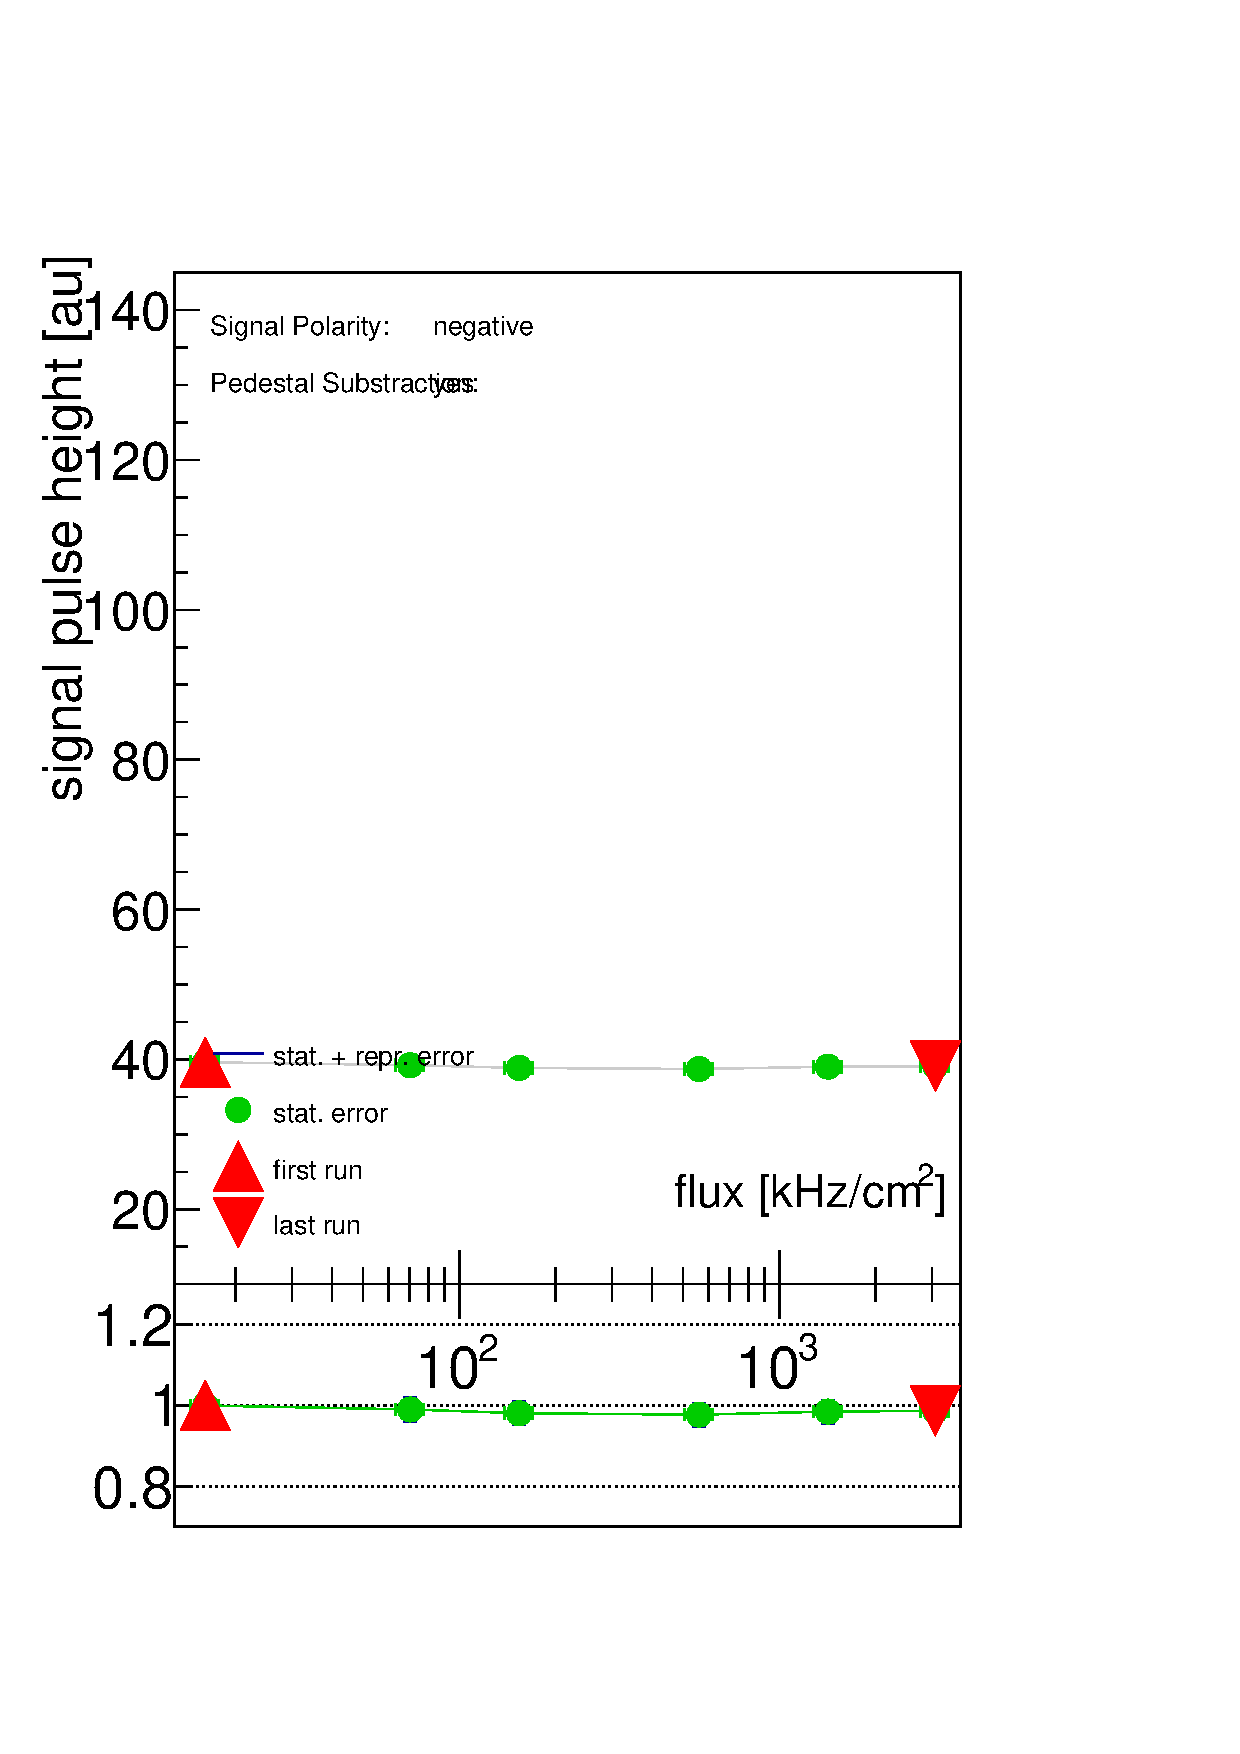
\includegraphics[width=3cm]{CPH1610_6_1.pdf}\\
		noise $\upsigma \approx$ \SI{4.9}{au}
	\end{minipage}\s
	\begin{itemize}
		\item pulse height very stable after irradiation
		\item noise stays the same
	\end{itemize}
\end{frame}


% ============= 6 =============
\section{3D Detectors}
\begin{frame}{Detector Concept}

	\vspace*{-10pt}
	\begin{figure} 
		\begin{center}
			\begin{subfigure}{0.4\textwidth}  
				\centering 
				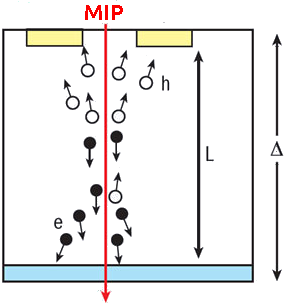
\includegraphics[height=.53\textheight]{PlanarConcept}
				\caption{planar detector}
			\end{subfigure}
			\begin{subfigure}{0.1\textwidth}  
				\centering 
				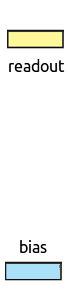
\includegraphics[height=.53\textheight]{LegendConcept}
				\vspace*{20pt}
			\end{subfigure}
			\begin{subfigure}{0.4\textwidth} 
				\centering 
				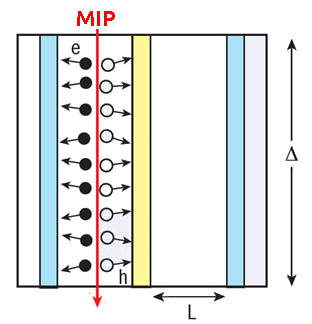
\includegraphics[height=.53\textheight]{3DConcept}
				\caption{3D detector} 	
			\end{subfigure} 
		\end{center}
	\end{figure}\vspace*{-10pt}
	
	\begin{itemize}
		\itemfill
		\item bias and readout electrode inside detector material
		\item same thickness $\Updelta$ \ra same amount of induced charge
		\item shorter drift distance L
		\item \usebeamercolor[fg]{title} \textbf{increase collected charge in detectors with limited mean free path}
	\end{itemize}
	
\end{frame}
% ================================== 2 =============================
\begin{frame}{3D Detector}
	
	\begin{figure}
		\centering
		\begin{subfigure}{0.4\textwidth}  
			\centering 
			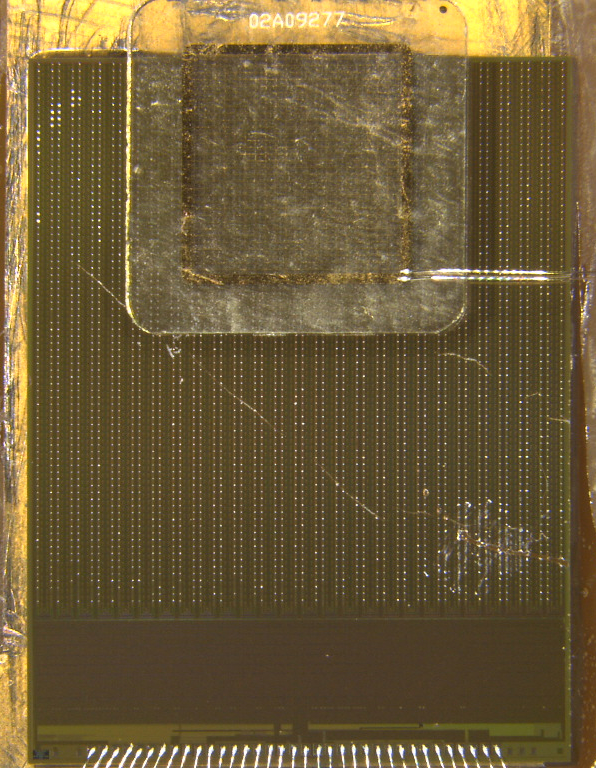
\includegraphics[height=.47\textheight]{Full3D}
			\caption{detector bonded on CMS pixel}
		\end{subfigure}
		\hspace*{10pt}
		\begin{subfigure}{0.4\textwidth} 
			\centering 
			\vspace*{.1\textheight}
			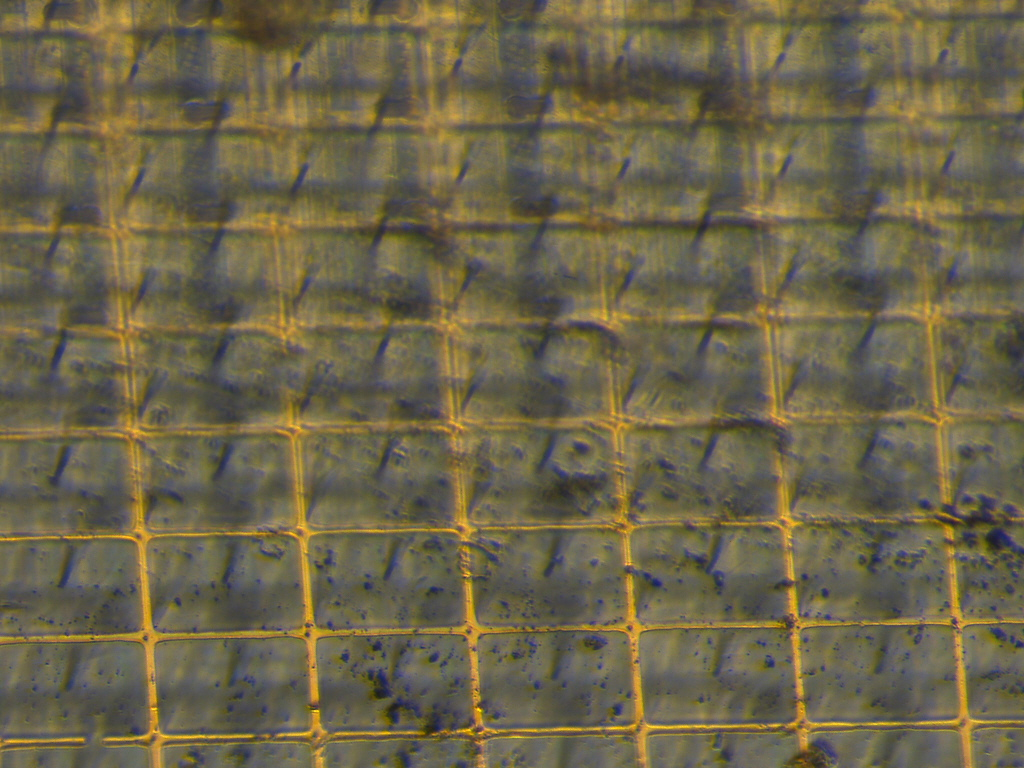
\includegraphics[height=.37\textheight]{3DCols}
			\caption{bias grid and columns}
		\end{subfigure}
	\end{figure}\vspace*{-10pt}

	\begin{itemize}
		\itemfill
		\item columns laser drilled \ra convert diamond into resistive mixture of carbon phases
		\item size of \SI{4x4}{\milli\meter}
		\item thickness of \SI{500}{\micro\meter}
		\item cell size of \SI{150x100}{\micro\meter} \ra \SI{20x30}{cells}
	\end{itemize}

\end{frame}
% ================================== 3 =============================
\begin{frame}{Raw Data}

	\vspace*{-10pt}
	\begin{figure}
		\centering
		\begin{subfigure}{0.45\textwidth}  
			\centering 
			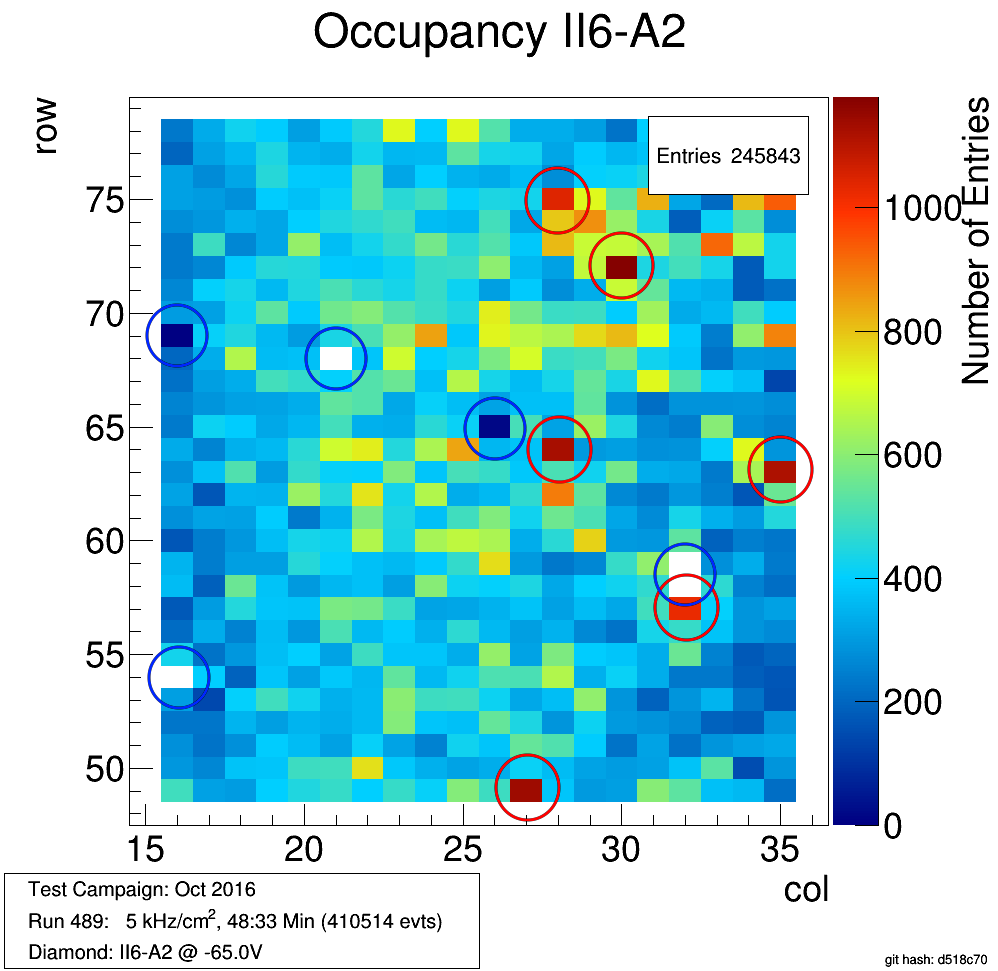
\includegraphics[height=.53\textheight]{OccRaw}
			\caption{raw hit map}
		\end{subfigure}
		\hspace*{10pt}
		\begin{subfigure}{0.45\textwidth} 
			\centering 
			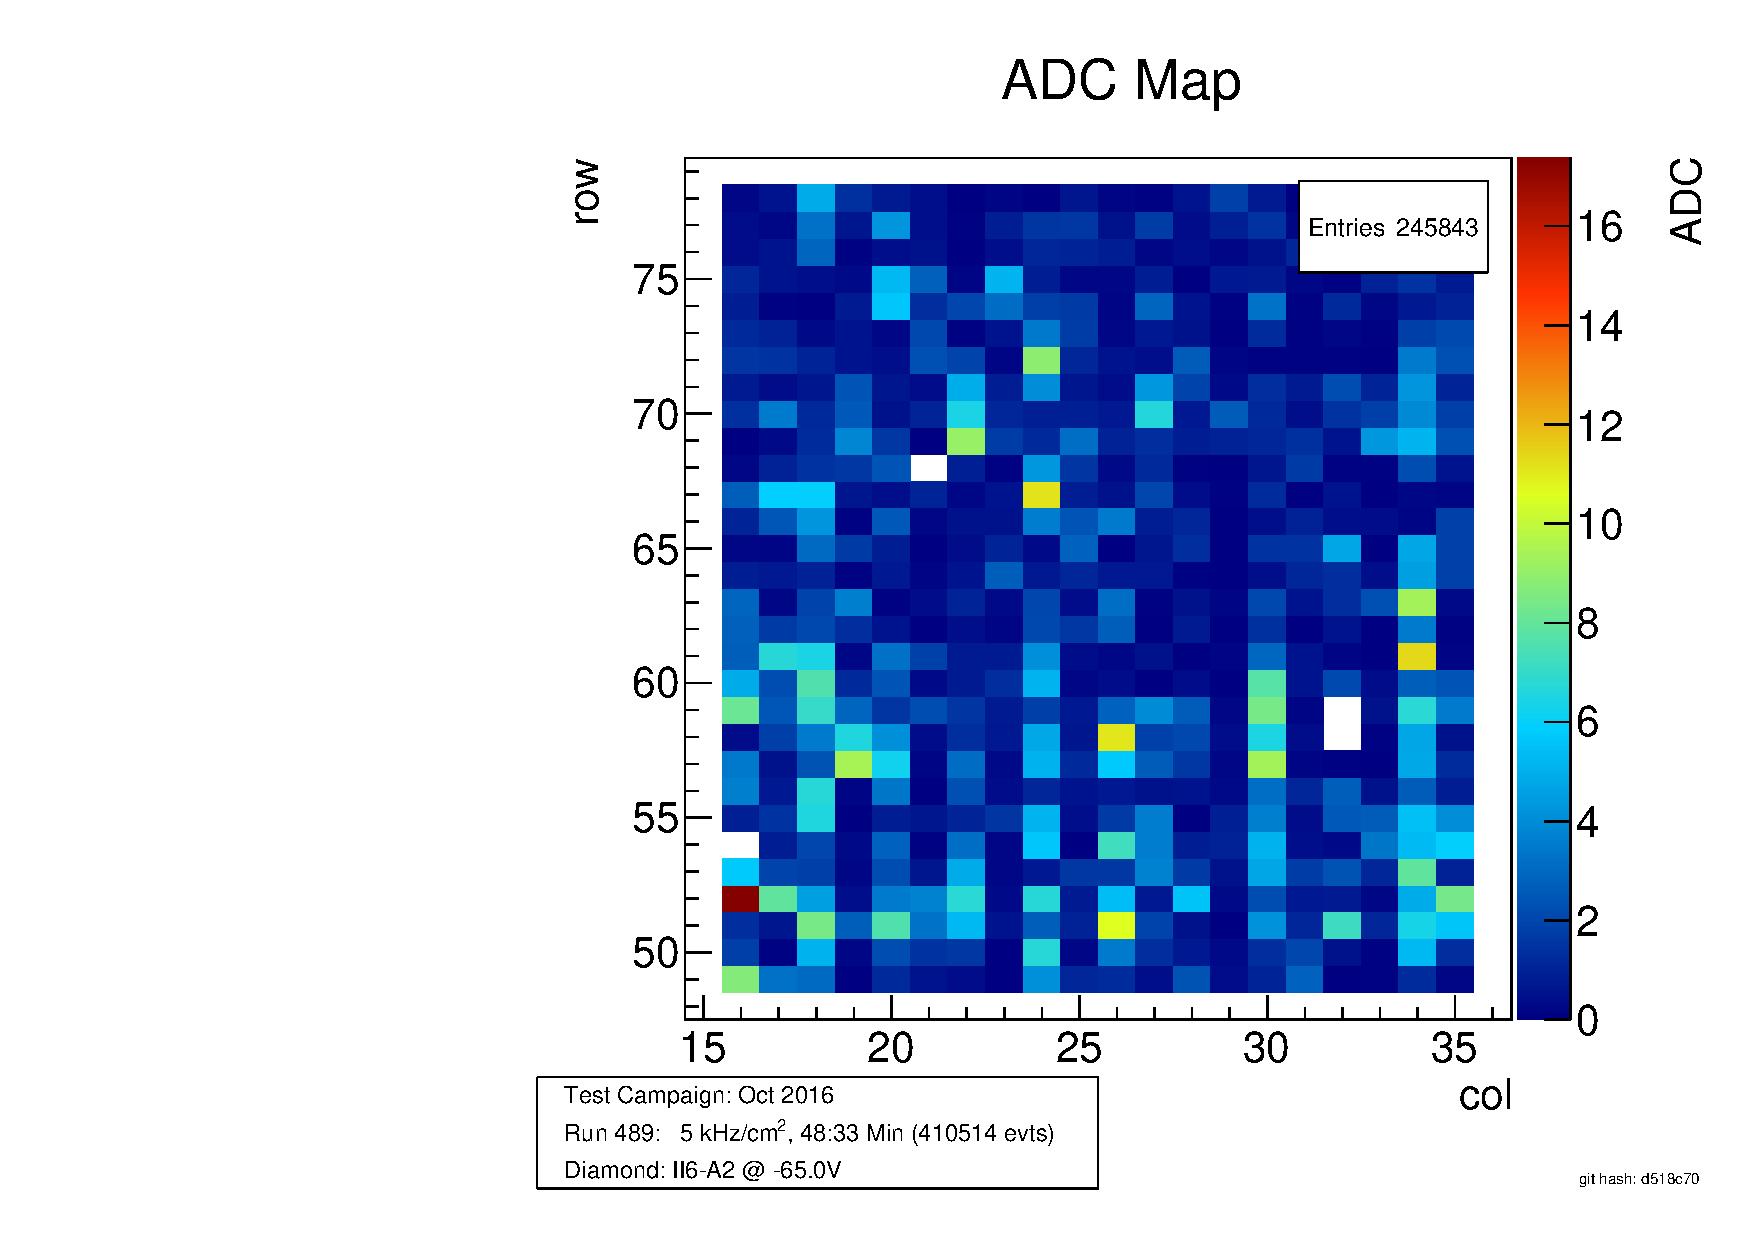
\includegraphics[width=.53\textheight, angle=-90]{AdcMapRaw}
			\caption{raw adc map}
		\end{subfigure}
	\end{figure}\vspace*{-10pt}
	
	\begin{itemize}
		\itemfill
		\item some hot (6) and dead (6) pixels in the detector (total 600 pixels)
		\item very low adc values (\SI{8}{bit} range) \ra most of the values are 0
		\item \textcolor{RedOrange}{\textbf{mistuned chip induced loss of pulse height information}}
	\end{itemize}

\end{frame}
% ================================== 4 ===============================================
\begin{frame}{Pulse Height Distribution}

	\vspace*{-10pt}
	\begin{figure} 
		\begin{center}
			\begin{subfigure}{0.48\textwidth}  
				\centering 
				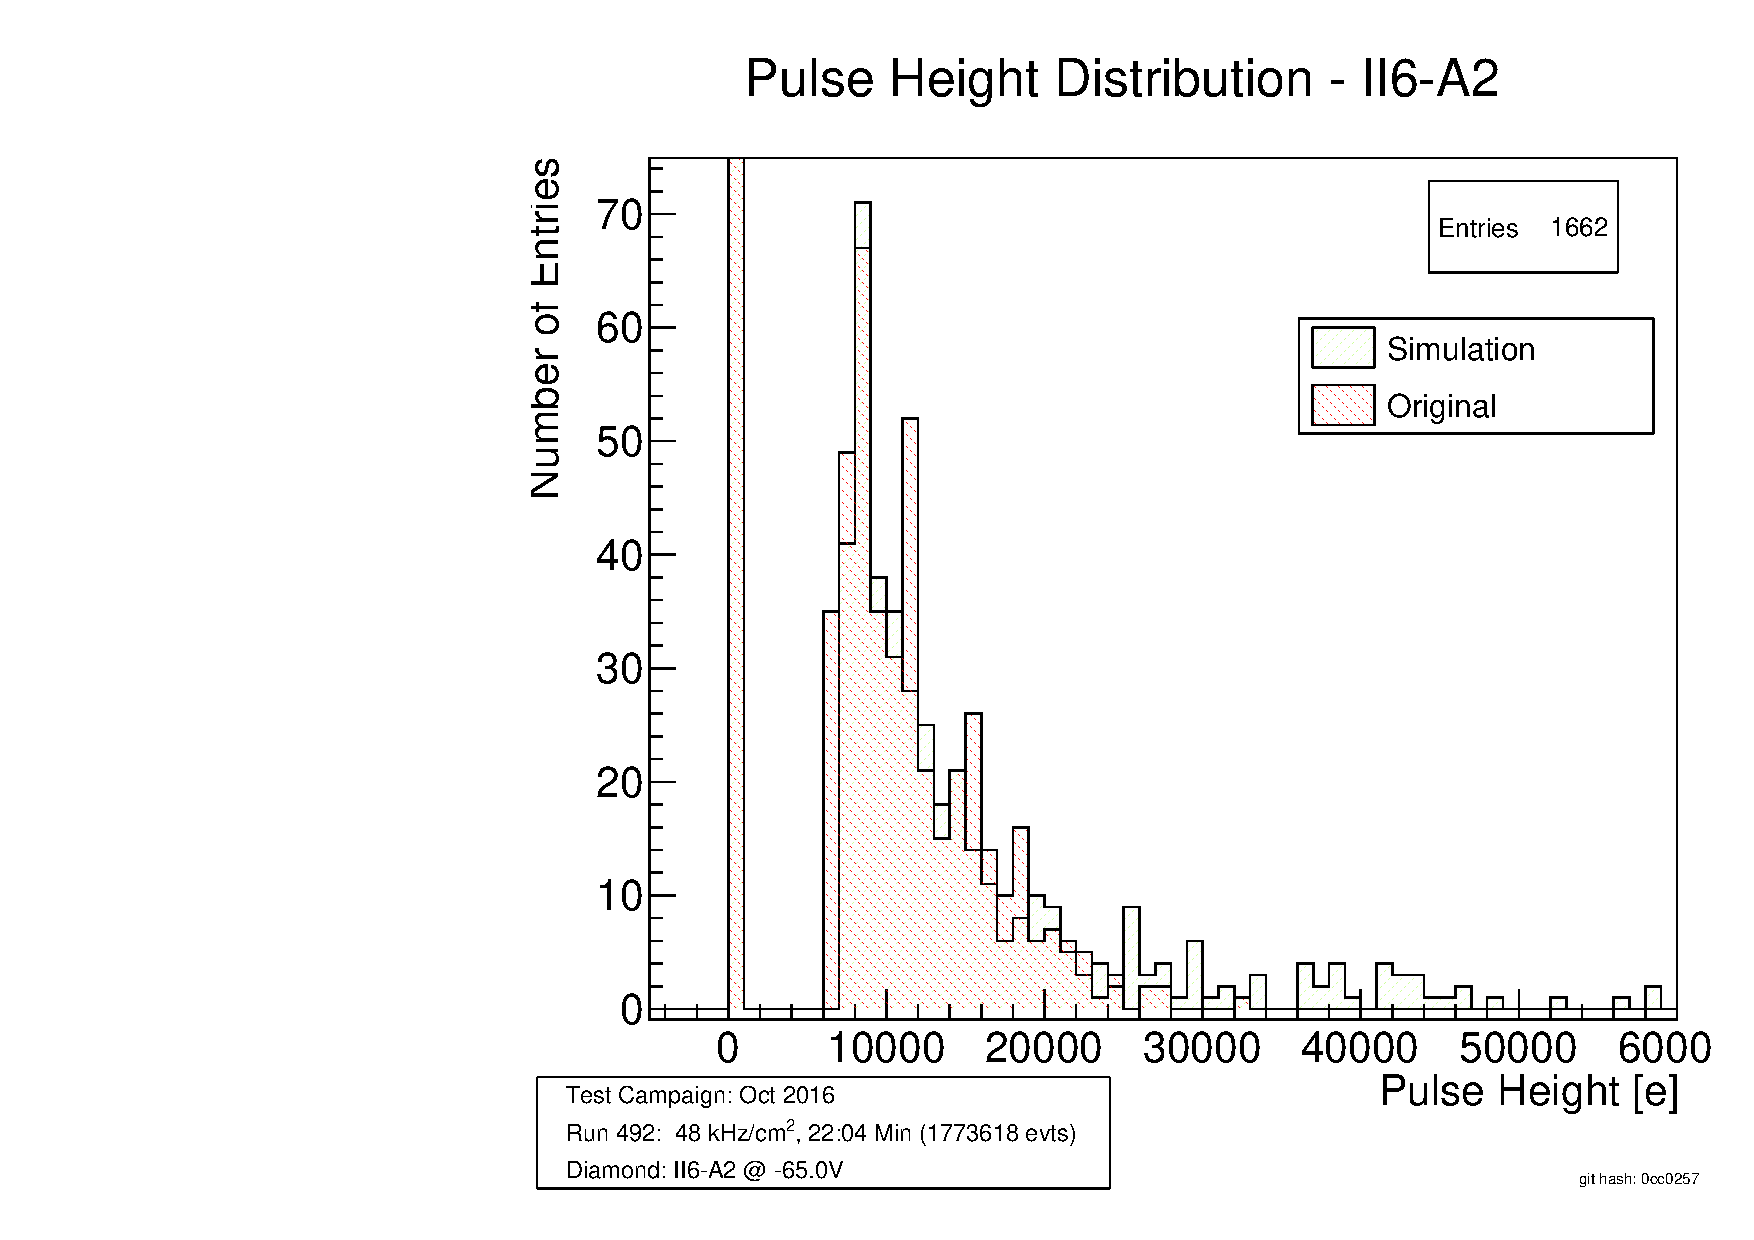
\includegraphics[height=.5\textheight, angle=-90]{Sim2}
				\caption{simulation of Landau with threshold} 	
			\end{subfigure}
			\begin{subfigure}{0.48\textwidth} 
				\centering 
				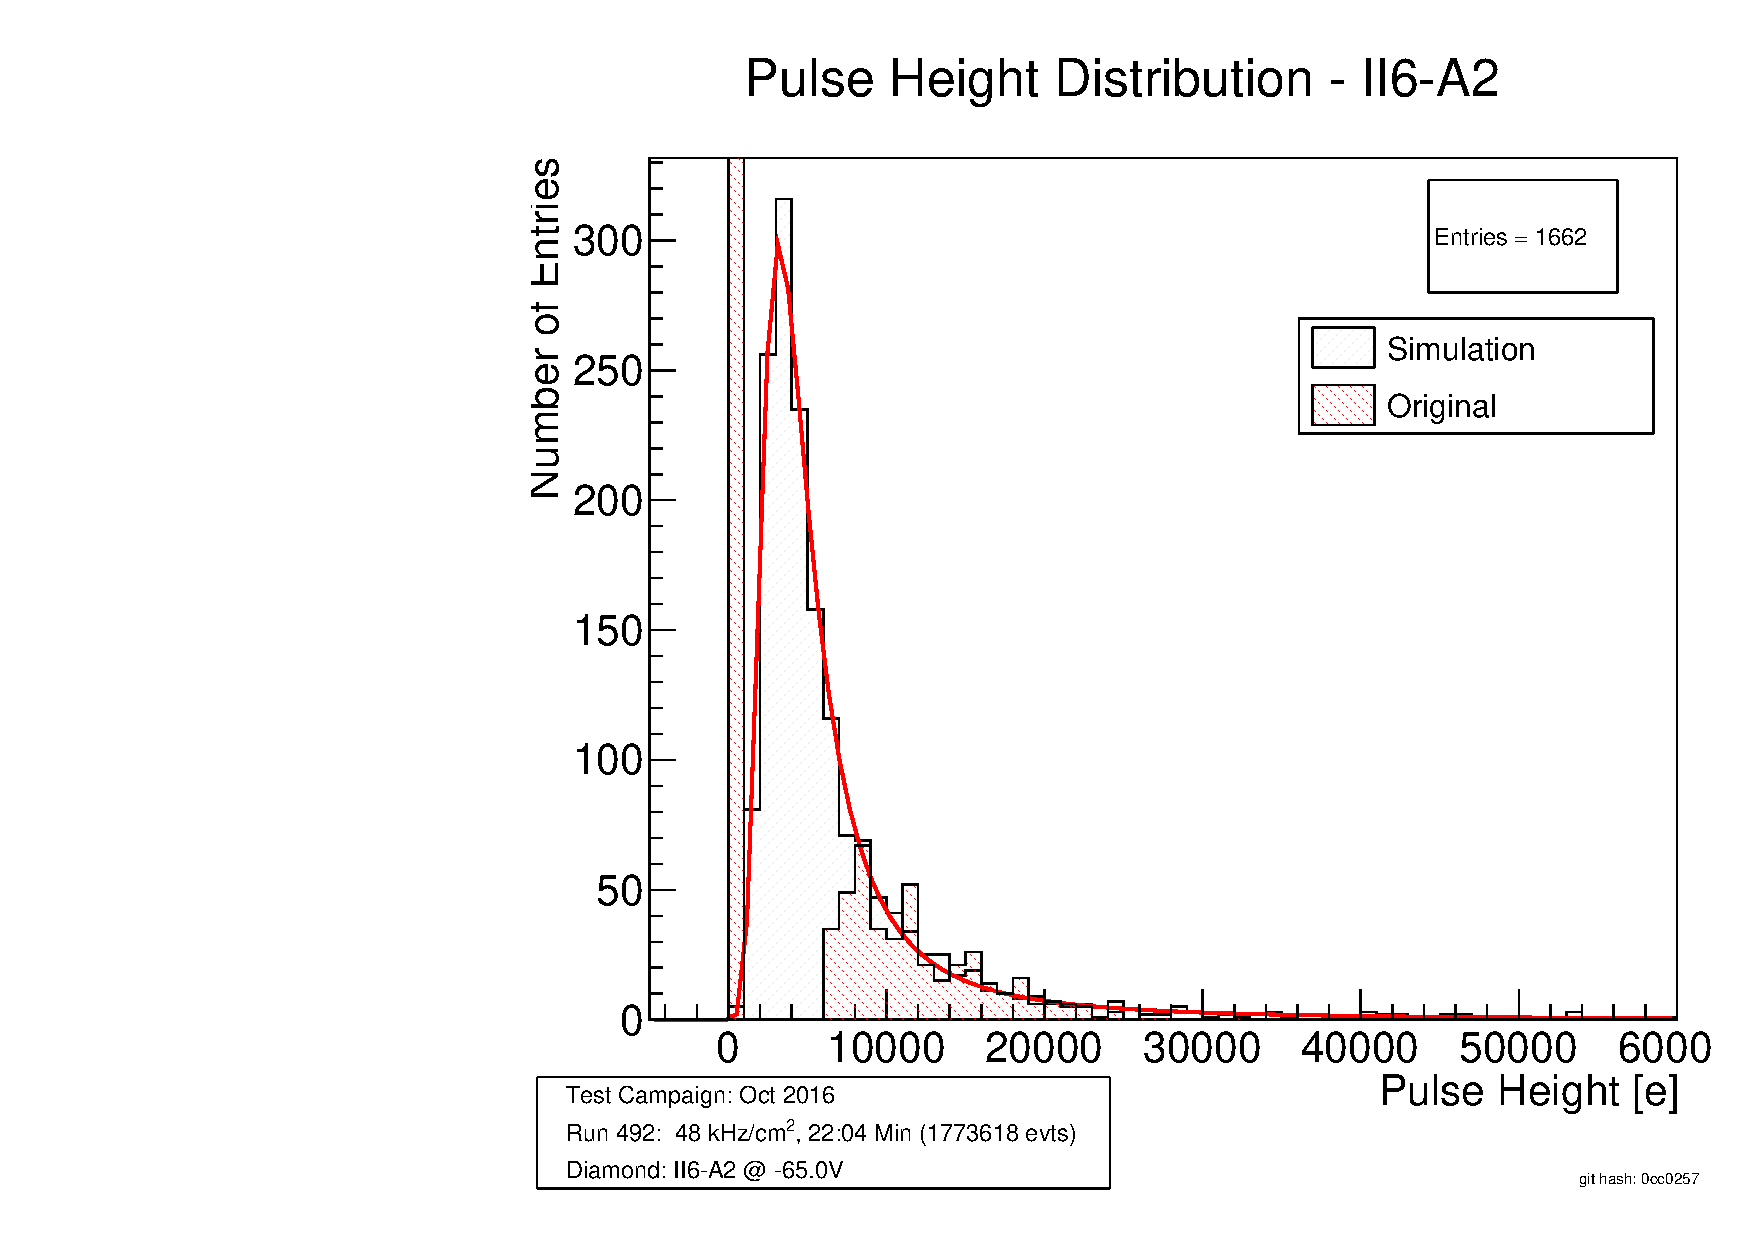
\includegraphics[height=.5\textheight, angle=-90]{Sim3}
				\caption{full distribution with fit} 	
			\end{subfigure} 
		\end{center}
	\end{figure}
	
	\begin{itemize}
		\itemfill
		\item \usebeamercolor[fg]{title} \textbf{mean of the full simulated distribution: \SI{6950}{e}}\usebeamercolor[fg]{normal text}
		\item lower than expected pulse height: \SI{>14000}{e} \ra under investigation
		\item \SI{1.8}{\%} of the events beneath \SI{1500}{e} (pixel threshold)
	\end{itemize}

\end{frame}
% ================================== 5 ===============================================
\begin{frame}{Efficiency Map}

	\vspace*{-10pt}
	\begin{figure} 
		\begin{center}
			\begin{subfigure}{0.48\textwidth}  
				\centering 
				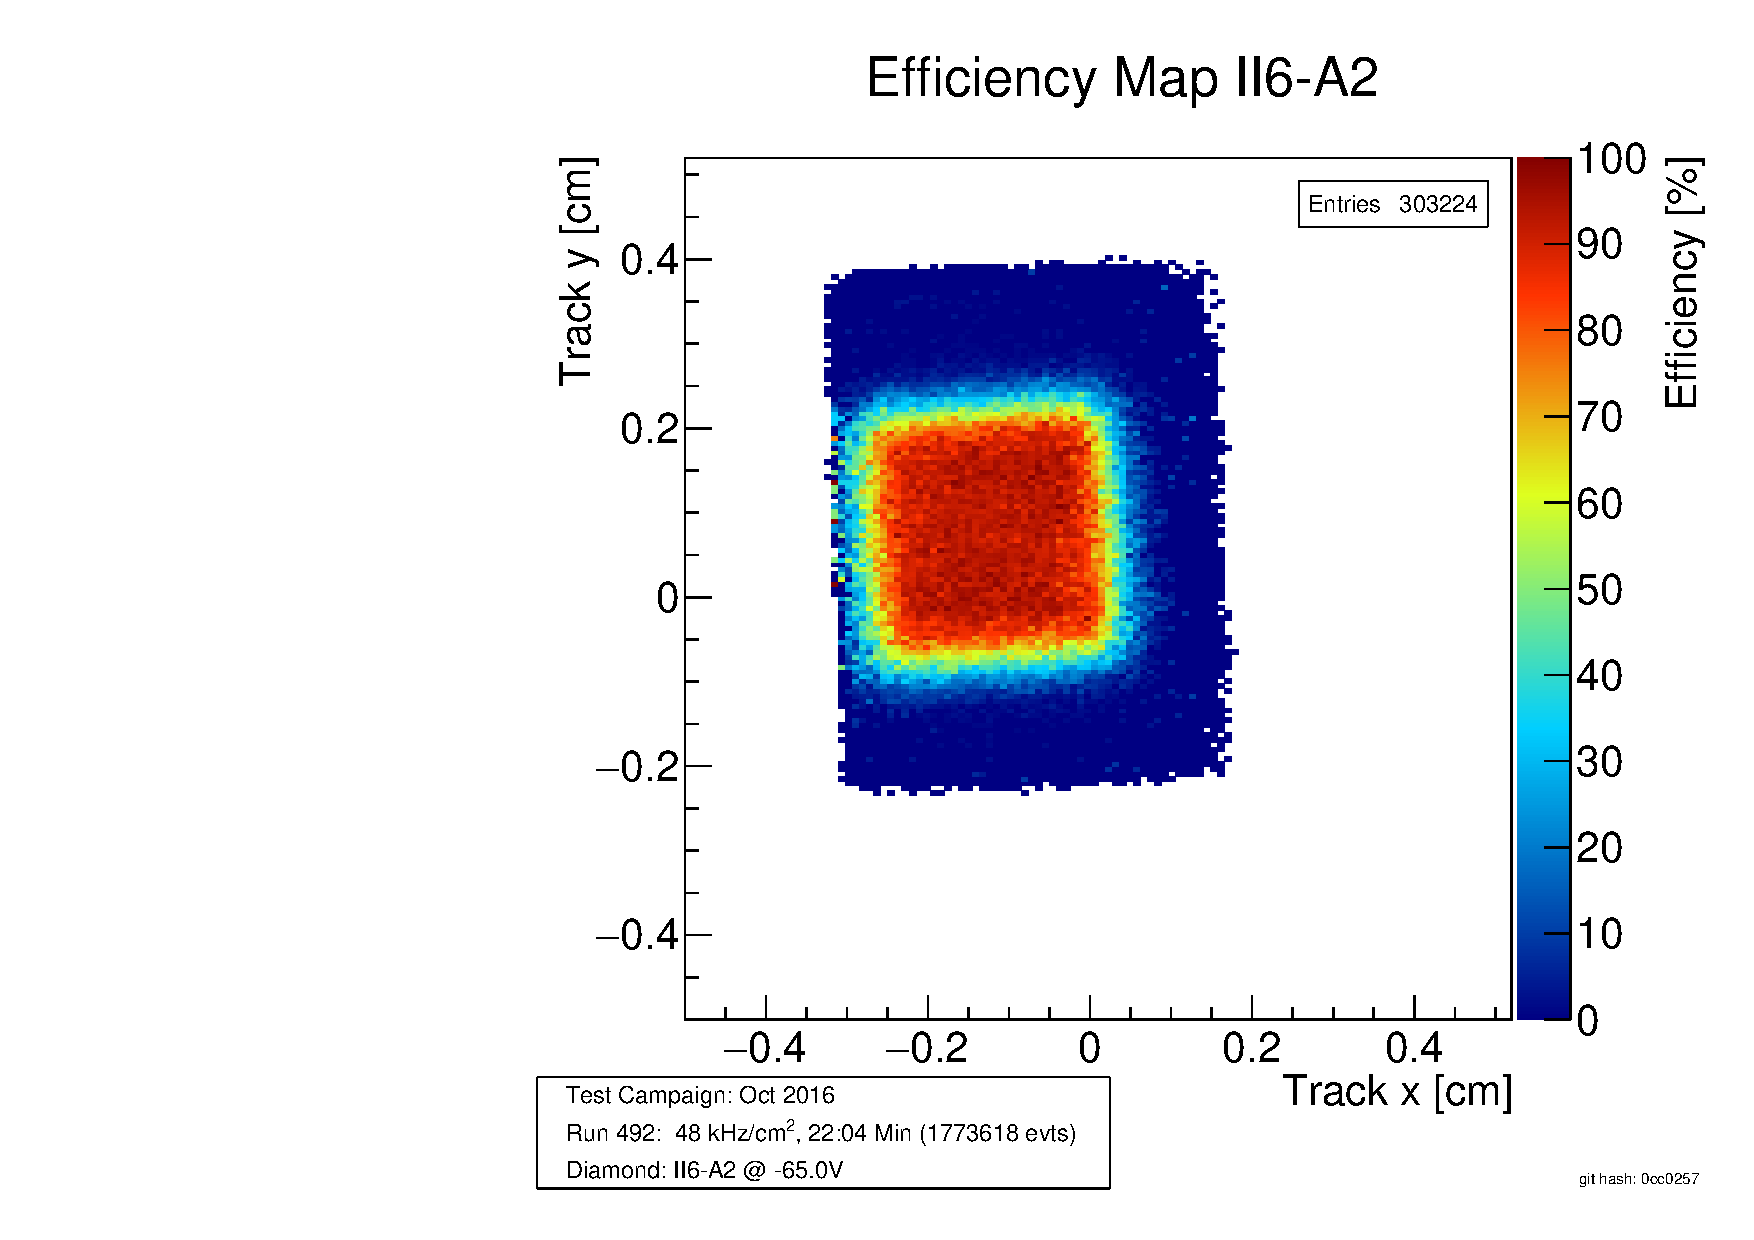
\includegraphics[height=.53\textheight, angle=-90]{EffMap}
				\caption{II6-A2} 	
			\end{subfigure}
			\begin{subfigure}{0.48\textwidth} 
				\centering 
				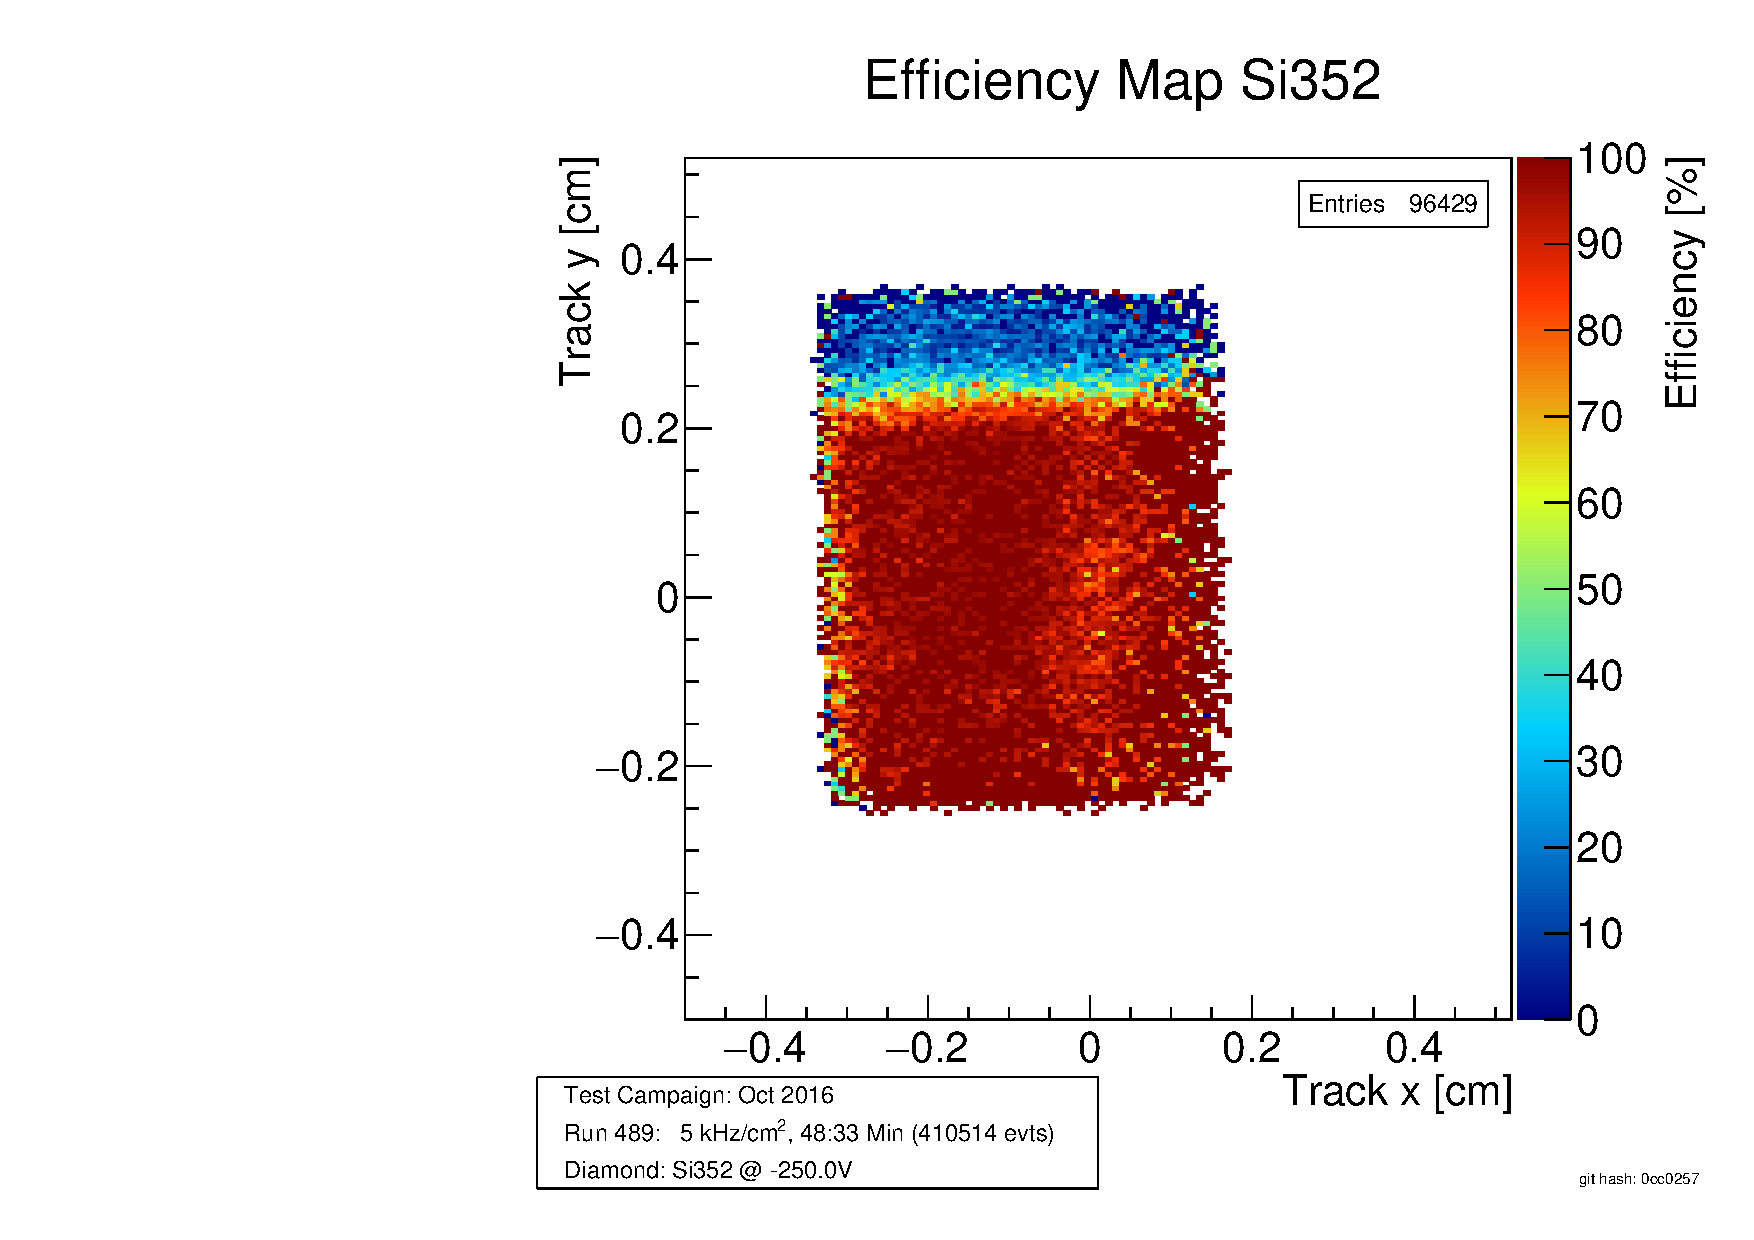
\includegraphics[height=.53\textheight, angle=-90]{EffMapSil}
				\caption{Si352 - reference} 	
			\end{subfigure} 
		\end{center}
	\end{figure}
	
	\begin{itemize}
		\itemfill
		\item percentage of valid hits at estimated hit position by tracking
		\item total area: unmasked area of the trigger planes
		\item central region highly efficient
	\end{itemize}

\end{frame}
% ================================== 6 ===============================================
\begin{frame}{Efficiency vs. Time}

	\vspace*{-10pt}
	\begin{figure} 
		\begin{center}
			\begin{subfigure}{0.48\textwidth}  
				\centering 
				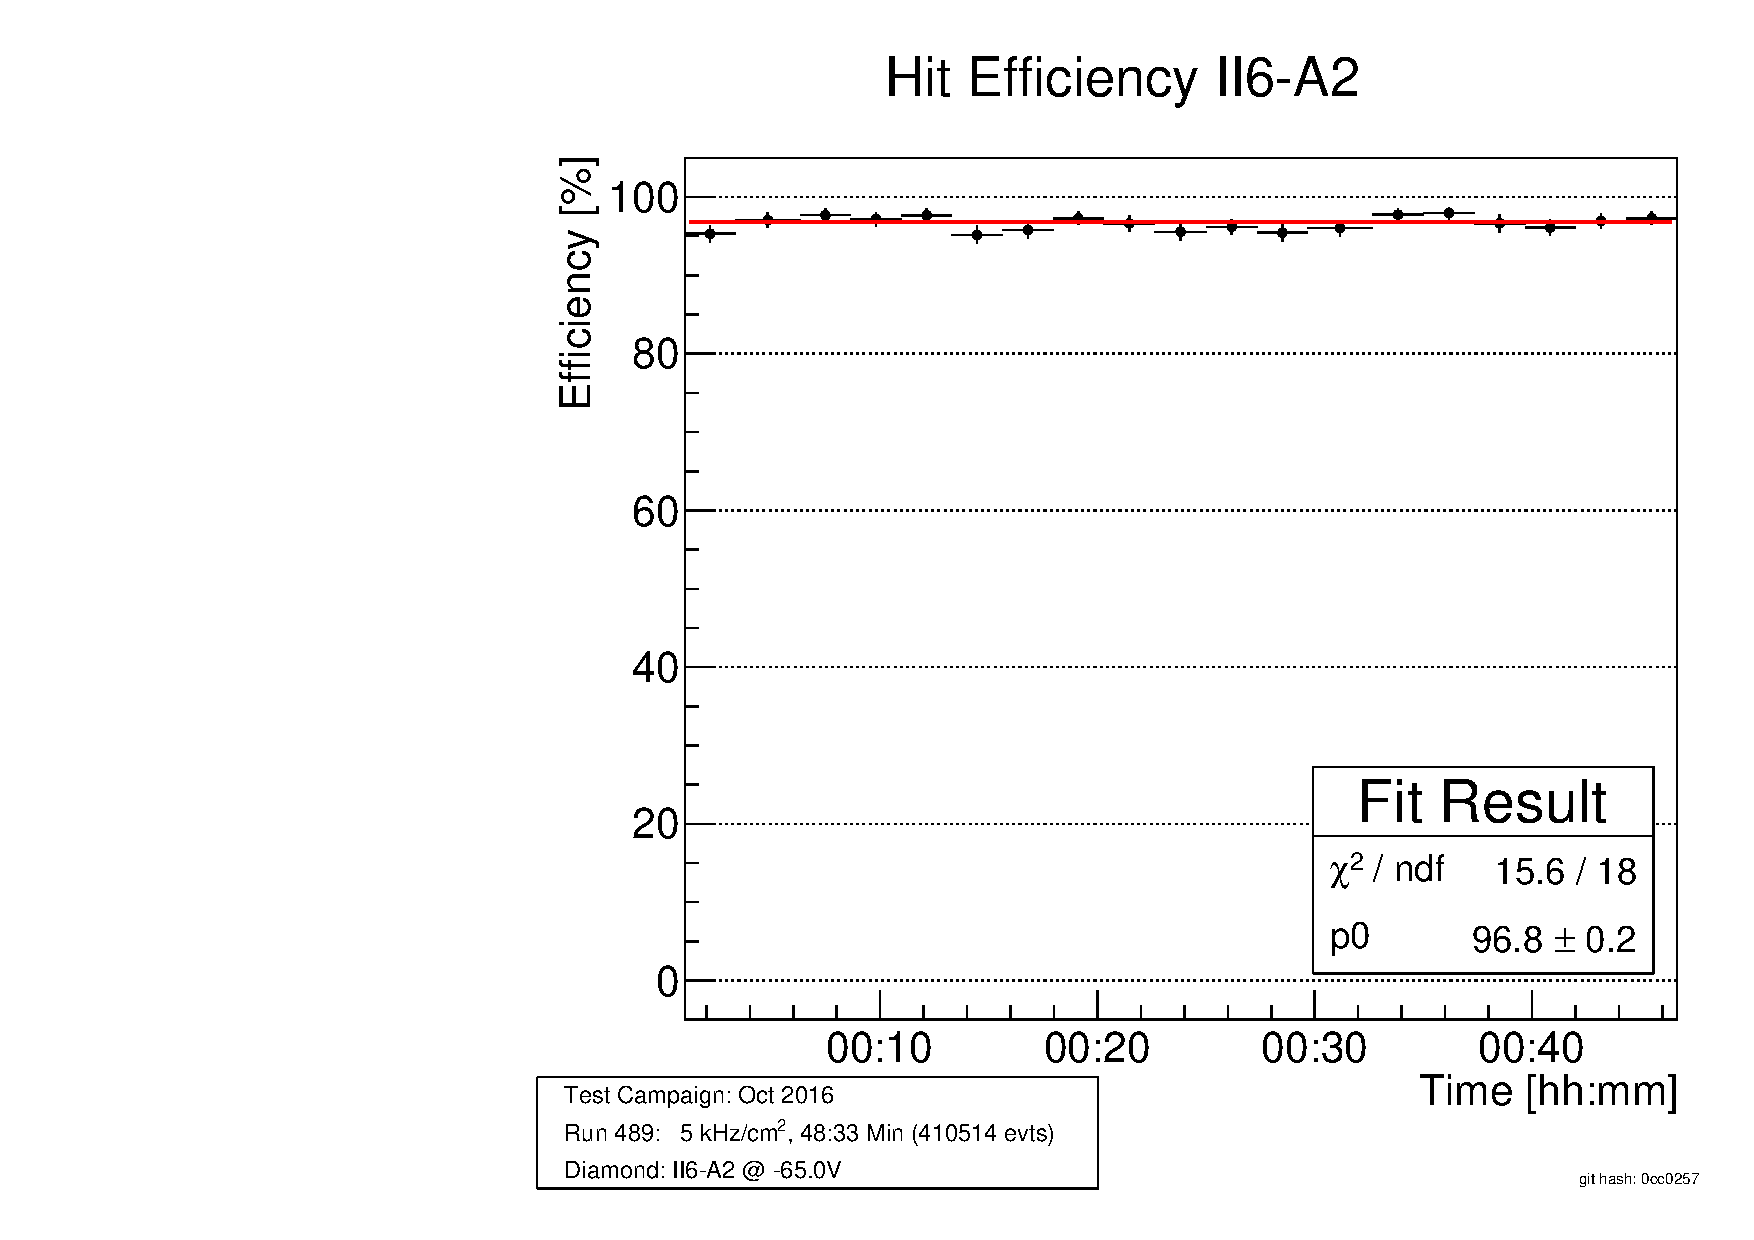
\includegraphics[height=.53\textheight, angle=-90]{EffDiaCut}
				\caption{II6-A2} 	
			\end{subfigure}
			\begin{subfigure}{0.48\textwidth} 
				\centering 
				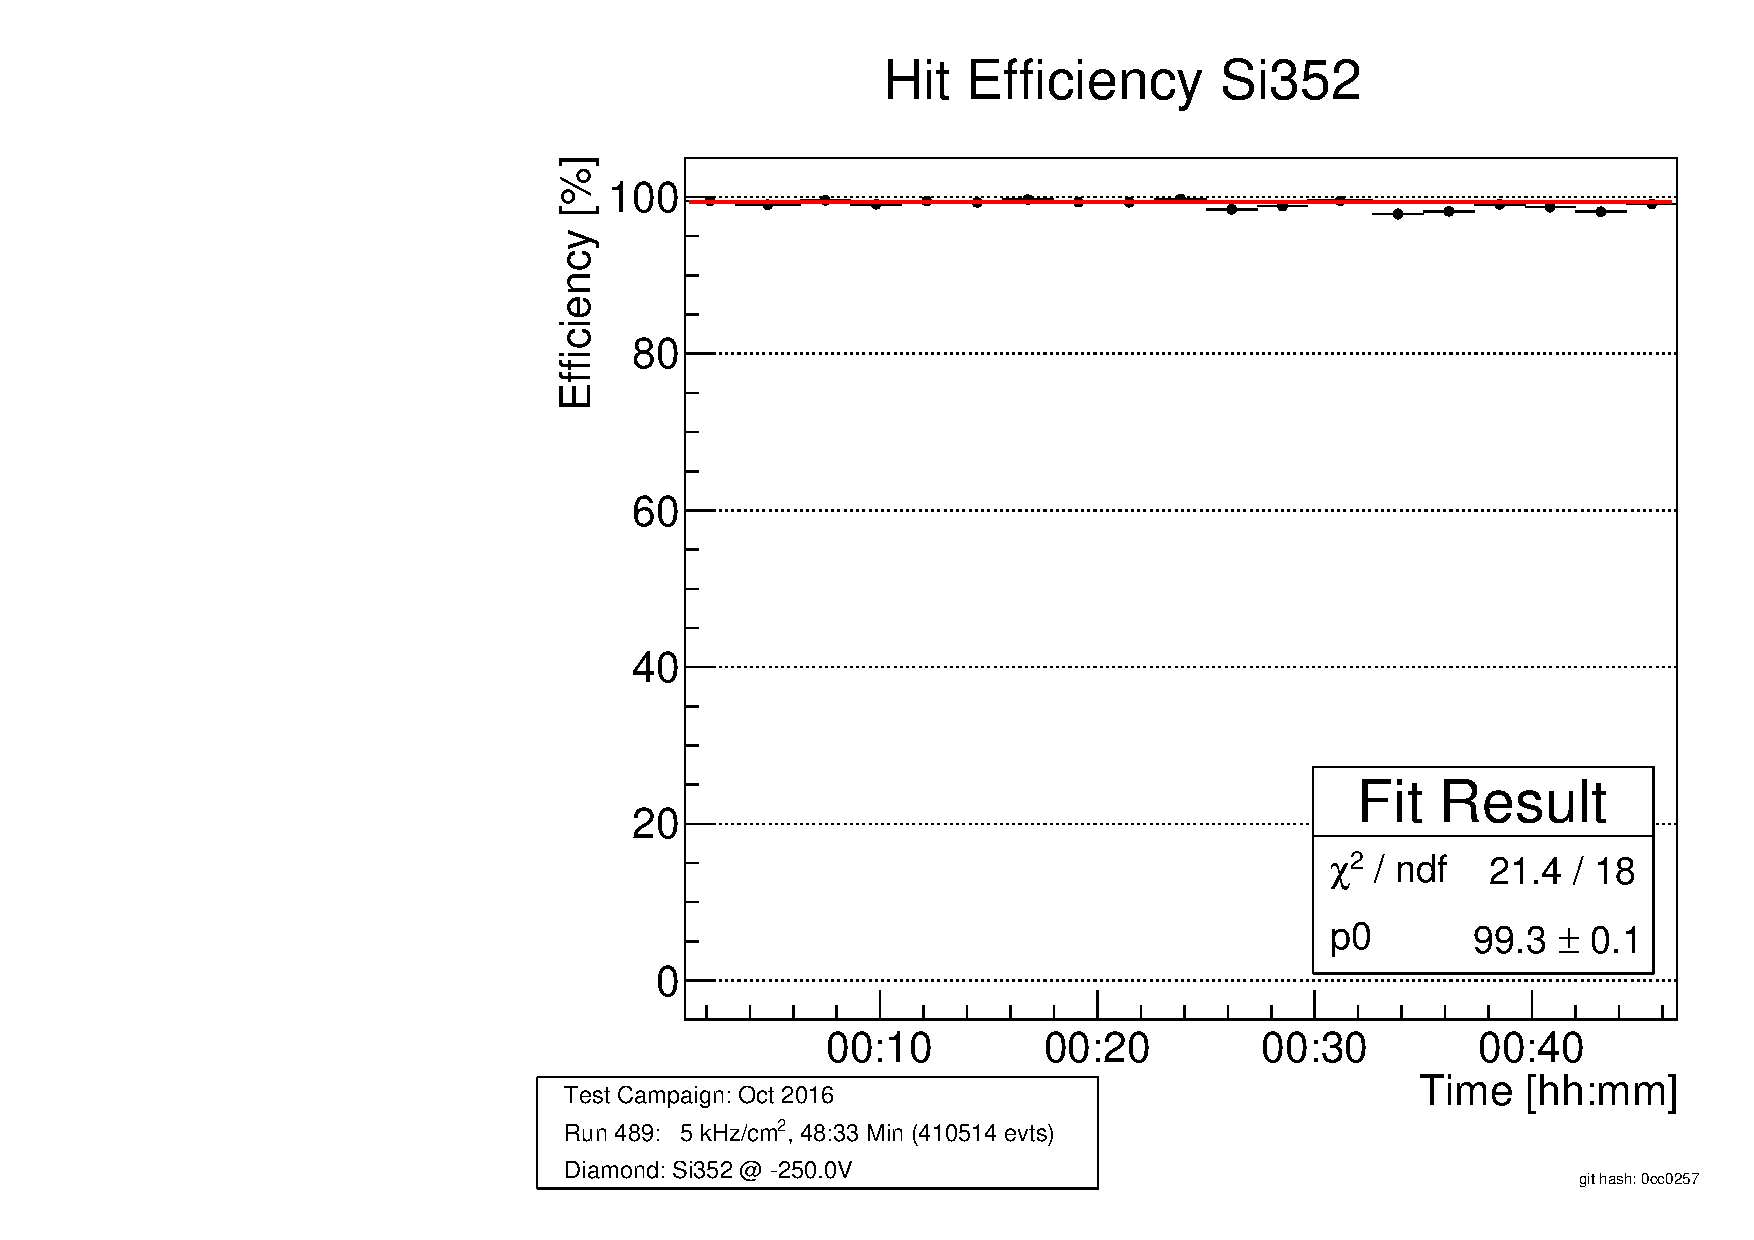
\includegraphics[height=.53\textheight, angle=-90]{EffSilCut}
				\caption{Si352 - reference} 	
			\end{subfigure} 
		\end{center}
	\end{figure}
	
	\begin{itemize}
		\itemfill
		\item \usebeamercolor[fg]{title} \textbf{mean efficiency of the II6-A2: \SI{\sim97}{\%}}\usebeamercolor[fg]{normal text}
		\item mean efficiency of the silicon reference: \SI{\sim99}{\%}
		\item undetected hits likely below pixel threshold \ra agrees well with simulation
	\end{itemize}

\end{frame}


% ============= 7 =============
\section{Pixel Detectors}
\begin{frame}{Pixel Detectors}

	\begin{figure}[h] 
		\centering
		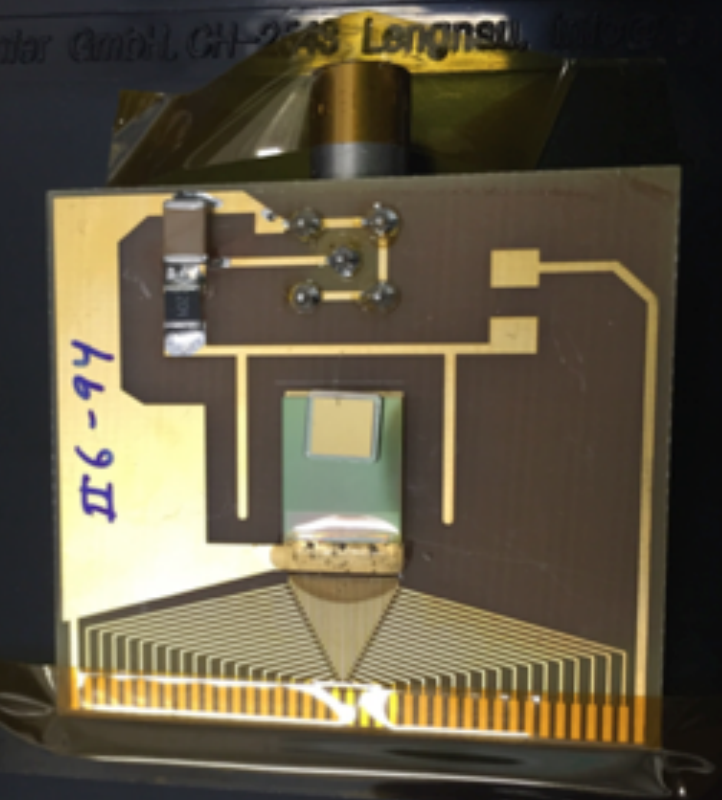
\includegraphics[height=0.5\textheight]{PixDet1}
		\caption{diamond sensor detector on CMS Pixel Chip} 	
	\end{figure}
	
	\begin{itemize}
		\itemfill
		\item cleaning, photo-lithography and Cr-Au metallisation at OSU and Princeton
		\item bump bonding at Princeton
		\item analysis very similar (easier) to 3D \ra ongoing
	\end{itemize}
	
\end{frame}


% ============= -1 =============
\section{Conclusion}
\begin{frame}
	\frametitle{Conclusion}
	\begin{minipage}[c][4cm]{\textwidth}
		\begin{itemize}
			\itemfill
			\item commissioned the ETH beam telescope
			\item designing new improved version of the telescope \ra soon to be tested
			\item pad analysis almost finished \ra paper soon
			\item started pixel analysis
			\item successfully measured the very first 3D diamond pixel detector
			\begin{itemize}
				\item high detecting efficiency of \SI{\sim97}{\%}
				\item very high pixel yield (only 6/600 dead pixels)
			\end{itemize}
		\end{itemize}
	\end{minipage}
\end{frame}


% DOCUMENT END
\end{document}

